\documentclass[a4paper]{book}
\usepackage{lmodern}
\usepackage{amssymb,amsmath}
\usepackage{ifxetex,ifluatex}
\usepackage{fixltx2e} % provides \textsubscript
\ifnum 0\ifxetex 1\fi\ifluatex 1\fi=0 % if pdftex
  \usepackage[T1]{fontenc}
  \usepackage[utf8]{inputenc}
\else % if luatex or xelatex
  \ifxetex
    \usepackage{mathspec}
  \else
    \usepackage{fontspec}
  \fi
  \defaultfontfeatures{Ligatures=TeX,Scale=MatchLowercase}
\fi
% use upquote if available, for straight quotes in verbatim environments
\IfFileExists{upquote.sty}{\usepackage{upquote}}{}
% use microtype if available
\IfFileExists{microtype.sty}{%
\usepackage{microtype}
\UseMicrotypeSet[protrusion]{basicmath} % disable protrusion for tt fonts
}{}
\usepackage[margin=1in]{geometry}
\usepackage{hyperref}
\hypersetup{unicode=true,
            pdftitle={Introduction to R},
            pdfauthor={QFAB},
            pdfborder={0 0 0},
            breaklinks=true}
\urlstyle{same}  % don't use monospace font for urls
\usepackage{natbib}
\bibliographystyle{plainnat}
\usepackage{color}
\usepackage{fancyvrb}
\newcommand{\VerbBar}{|}
\newcommand{\VERB}{\Verb[commandchars=\\\{\}]}
\DefineVerbatimEnvironment{Highlighting}{Verbatim}{commandchars=\\\{\}}
% Add ',fontsize=\small' for more characters per line
\usepackage{framed}
\definecolor{shadecolor}{RGB}{248,248,248}
\newenvironment{Shaded}{\begin{snugshade}}{\end{snugshade}}
\newcommand{\KeywordTok}[1]{\textcolor[rgb]{0.13,0.29,0.53}{\textbf{{#1}}}}
\newcommand{\DataTypeTok}[1]{\textcolor[rgb]{0.13,0.29,0.53}{{#1}}}
\newcommand{\DecValTok}[1]{\textcolor[rgb]{0.00,0.00,0.81}{{#1}}}
\newcommand{\BaseNTok}[1]{\textcolor[rgb]{0.00,0.00,0.81}{{#1}}}
\newcommand{\FloatTok}[1]{\textcolor[rgb]{0.00,0.00,0.81}{{#1}}}
\newcommand{\ConstantTok}[1]{\textcolor[rgb]{0.00,0.00,0.00}{{#1}}}
\newcommand{\CharTok}[1]{\textcolor[rgb]{0.31,0.60,0.02}{{#1}}}
\newcommand{\SpecialCharTok}[1]{\textcolor[rgb]{0.00,0.00,0.00}{{#1}}}
\newcommand{\StringTok}[1]{\textcolor[rgb]{0.31,0.60,0.02}{{#1}}}
\newcommand{\VerbatimStringTok}[1]{\textcolor[rgb]{0.31,0.60,0.02}{{#1}}}
\newcommand{\SpecialStringTok}[1]{\textcolor[rgb]{0.31,0.60,0.02}{{#1}}}
\newcommand{\ImportTok}[1]{{#1}}
\newcommand{\CommentTok}[1]{\textcolor[rgb]{0.56,0.35,0.01}{\textit{{#1}}}}
\newcommand{\DocumentationTok}[1]{\textcolor[rgb]{0.56,0.35,0.01}{\textbf{\textit{{#1}}}}}
\newcommand{\AnnotationTok}[1]{\textcolor[rgb]{0.56,0.35,0.01}{\textbf{\textit{{#1}}}}}
\newcommand{\CommentVarTok}[1]{\textcolor[rgb]{0.56,0.35,0.01}{\textbf{\textit{{#1}}}}}
\newcommand{\OtherTok}[1]{\textcolor[rgb]{0.56,0.35,0.01}{{#1}}}
\newcommand{\FunctionTok}[1]{\textcolor[rgb]{0.00,0.00,0.00}{{#1}}}
\newcommand{\VariableTok}[1]{\textcolor[rgb]{0.00,0.00,0.00}{{#1}}}
\newcommand{\ControlFlowTok}[1]{\textcolor[rgb]{0.13,0.29,0.53}{\textbf{{#1}}}}
\newcommand{\OperatorTok}[1]{\textcolor[rgb]{0.81,0.36,0.00}{\textbf{{#1}}}}
\newcommand{\BuiltInTok}[1]{{#1}}
\newcommand{\ExtensionTok}[1]{{#1}}
\newcommand{\PreprocessorTok}[1]{\textcolor[rgb]{0.56,0.35,0.01}{\textit{{#1}}}}
\newcommand{\AttributeTok}[1]{\textcolor[rgb]{0.77,0.63,0.00}{{#1}}}
\newcommand{\RegionMarkerTok}[1]{{#1}}
\newcommand{\InformationTok}[1]{\textcolor[rgb]{0.56,0.35,0.01}{\textbf{\textit{{#1}}}}}
\newcommand{\WarningTok}[1]{\textcolor[rgb]{0.56,0.35,0.01}{\textbf{\textit{{#1}}}}}
\newcommand{\AlertTok}[1]{\textcolor[rgb]{0.94,0.16,0.16}{{#1}}}
\newcommand{\ErrorTok}[1]{\textcolor[rgb]{0.64,0.00,0.00}{\textbf{{#1}}}}
\newcommand{\NormalTok}[1]{{#1}}
\usepackage{longtable,booktabs}
\usepackage{graphicx,grffile}
\makeatletter
\def\maxwidth{\ifdim\Gin@nat@width>\linewidth\linewidth\else\Gin@nat@width\fi}
\def\maxheight{\ifdim\Gin@nat@height>\textheight\textheight\else\Gin@nat@height\fi}
\makeatother
% Scale images if necessary, so that they will not overflow the page
% margins by default, and it is still possible to overwrite the defaults
% using explicit options in \includegraphics[width, height, ...]{}
\setkeys{Gin}{width=\maxwidth,height=\maxheight,keepaspectratio}
\IfFileExists{parskip.sty}{%
\usepackage{parskip}
}{% else
\setlength{\parindent}{0pt}
\setlength{\parskip}{6pt plus 2pt minus 1pt}
}
\setlength{\emergencystretch}{3em}  % prevent overfull lines
\providecommand{\tightlist}{%
  \setlength{\itemsep}{0pt}\setlength{\parskip}{0pt}}
\setcounter{secnumdepth}{5}
% Redefines (sub)paragraphs to behave more like sections
\ifx\paragraph\undefined\else
\let\oldparagraph\paragraph
\renewcommand{\paragraph}[1]{\oldparagraph{#1}\mbox{}}
\fi
\ifx\subparagraph\undefined\else
\let\oldsubparagraph\subparagraph
\renewcommand{\subparagraph}[1]{\oldsubparagraph{#1}\mbox{}}
\fi
\usepackage{booktabs}
\usepackage{longtable}
\usepackage{framed,color}
\usepackage{fancyhdr}
\definecolor{shadecolor}{RGB}{248,248,248}

%% set header and footer for PDF doc
\pagestyle{fancy}
\fancyhead[LO,RE]{}
\fancyfoot[LE,RO]{QFAB Bioinformatics | QCIF}
\fancyfoot[LO,RE]{\thepage}
\fancyfoot[CO,CE]{}

%% redefine some styles
%\setlength{\parskip}{1em}

\makeatletter
\def\@xobeysp{\mbox{}\space}
\def\verbatim@font{\normalfont\ttfamily\raggedright\leftskip\@totalleftmargin\vspace{-1em}}
\makeatother

\renewenvironment{Shaded}
{\vspace{1.5em}\begin{leftbar}\begin{snugshade}}
{\end{snugshade}\end{leftbar}\vspace{3pt}}

\definecolor{shadecolor}{RGB}{235,235,235}


%% custom boxes from bookdown
\ifxetex
  \usepackage{letltxmacro}
  \setlength{\XeTeXLinkMargin}{1pt}
  \LetLtxMacro\SavedIncludeGraphics\includegraphics
  \def\includegraphics#1#{% #1 catches optional stuff (star/opt. arg.)
    \IncludeGraphicsAux{#1}%
  }%
  \newcommand*{\IncludeGraphicsAux}[2]{%
    \XeTeXLinkBox{%
      \SavedIncludeGraphics#1{#2}%
    }%
  }%
\fi

\newenvironment{rmdblock}[1]
  {\vspace{1.5em}\begin{shaded*}
  \begin{itemize}
  \renewcommand{\labelitemi}{
    \raisebox{-.7\height}[0pt][0pt]{
      {\setkeys{Gin}{width=3em,keepaspectratio}\includegraphics{images/#1}}
    }
  }
  \item
  }
  {
  \end{itemize}
  \end{shaded*}
  }
\newenvironment{rmdnote}
  {\begin{rmdblock}{note}}
  {\end{rmdblock}}
\newenvironment{rmdcaution}
  {\begin{rmdblock}{caution}}
  {\end{rmdblock}}
\newenvironment{rmdimportant}
  {\begin{rmdblock}{important}}
  {\end{rmdblock}}
\newenvironment{rmdtip}
  {\begin{rmdblock}{tip}}
  {\end{rmdblock}}
\newenvironment{rmdwarning}
  {\begin{rmdblock}{warning}}
  {\end{rmdblock}}
\newenvironment{rmdexercise}
  {\begin{rmdblock}{exercise}}
  {\end{rmdblock}}

%%% Use protect on footnotes to avoid problems with footnotes in titles
\let\rmarkdownfootnote\footnote%
\def\footnote{\protect\rmarkdownfootnote}

%%% Change title format to be more compact
\usepackage{titling}

% Create subtitle command for use in maketitle
\newcommand{\subtitle}[1]{
  \posttitle{
    \begin{center}\large#1\end{center}
    }
}

\setlength{\droptitle}{-2em}
  \title{Introduction to R}
  \pretitle{\vspace{\droptitle}\centering\huge}
  \posttitle{\par}
  \author{QFAB}
  \preauthor{\centering\large\emph}
  \postauthor{\par}
  \date{}
  \predate{}\postdate{}

\begin{document}
\maketitle

{
\setcounter{tocdepth}{1}
\tableofcontents
}
\chapter*{Abstract}\label{abstract}
\addcontentsline{toc}{chapter}{Abstract}

R is a open-sourced software programming language and software
environment for statistical computing and graphics. The R language is
widely used among statisticians and data analysts for developing
statistical workflows for data analysis. R is an implementation of the S
programming language combined with lexical scoping semantics inspired by
Scheme. R was created by Ross Ihaka and Robert Gentleman at the
University of Auckland, New Zealand, and is currently developed by the R
Development Core Team.

Bioconductor is a project to develop innovative software tools for use
in computational biology. It is based on the R language. Bioconductor
packages provide flexible interactive tools for carrying out a number of
different computational tasks. Literate programming and analytical
pipeline crafting.

R and Bioconductor may not be as fast as dedicated bioinformatics
software for computationally intensive processes such as mapping short
sequence reads onto the genome, but the flexibility of having raw access
to all of the data, methods and structure is empowering.

\chapter{Getting started}\label{getting-started}

R is a statistical environment and programming language for data
analysis and graphical display. The software is open-source, freely
available and has been compiled ready for use on Windows, Mac and Linux
computers. The Bioconductor framework has a considerable number of
packages that have been implemented for the analysis and exploration of
metabolomics, proteomics, DNA microarray and Next Generation DNA
sequence data.

This workshop is intended as an introduction to R that should
familiarise you with the concepts that underpin the crafting of
workflows in R and some of the key techniques that will aid in the
crafting of reusable workflows.

Some of the topics we will cover over the course of the day include:

\begin{itemize}
\tightlist
\item
  Using the RStudio IDE for running a data analysis in R
\item
  The basics of literate programming for studies using R
\item
  Loading, creating, modifying and saving basic -omics data objects
  according to key formats
\item
  Create graphs and plots of data
\item
  Understanding how to read and understand someone else's R-code
\end{itemize}

\section{How to read this book}\label{how-to-read-this-book}

In the shaded dialog boxes with the thick left border are commands that
should be typed into your R \emph{Console} window. This corresponds to
\textbf{input}, the \textbf{output} will sometimes follow below with
lines preceeded with two hashmarks (\#\#).

\begin{Shaded}
\begin{Highlighting}[]
\KeywordTok{print}\NormalTok{(}\StringTok{"HELLO WORLD"}\NormalTok{)}
\end{Highlighting}
\end{Shaded}

\begin{verbatim}
## [1] "HELLO WORLD"
\end{verbatim}

\begin{rmdtip}
\textbf{Tips, Suggestions and Traps}

Comments and salient advice are provided in dialogs such as this. We'll
use this format to warn you of traps that you could slip into and to
provide some hints.
\end{rmdtip}

\begin{rmdcaution}
\textbf{Warnings and Traps}

Warnings are provided in dialogs such as this. We'll use this format to
warn you of traps that you could slip into and to provide some hints.
\end{rmdcaution}

\begin{rmdexercise}
\textbf{Time for you to make R work}

Exercises are the best way to learn. A document can provide an insight
to the process but hands-on interaction with R is the only way to learn.
In the exercise boxes are some suggested exercises that will apply the
knowledge that is being shared.
\end{rmdexercise}

\section{RStudio IDE}\label{rstudio-ide}

RStudio is a free and open source integrated development environment
(IDE) for R. An IDE is most typically used in software development where
a user is presented with a unified environment where code can be edited,
documentation can be read and debuggers can be applied to understand
what is happening in the code and why it may not be working as expected.

In bioinformatics (or computational biology) an IDE provides us with an
integrated approach to writing R scripts (or markdown documents),
interacting with our data as we implement our script and provides us
with an overview of the objects that we have created and their content.
RStudio also retains a history of the commands that we have typed, a
collection of the figures that we have prepared and provides access to
method documentation and package vignettes. We will consider all of
these aspects during this workshop. The RStudio IDE is great for the
preparation of scripts and reports since the code syntax-highlighting
helps you discover typos and errors in your code and even spelling
mistakes.

RStudio comes in two main flavours: a \emph{Desktop} version that runs
straight off the computer that we are sitting at and a \emph{Server}
version that can be hosted on a slightly more capable computer in a data
centre. The server version is sometimes preferable since it is accessed
via a web-browser and can be configured with massive memory and disk
allocations that might not be practical for a normal laptop. The server
version is platform-agnostic (from the user perspective that is; the
server itself needs to run Linux) and the Desktop version can be run on
Windows, Mac and Linux computers. An example RStudio session running on
the Desktop version is shown in Figure \ref{fig:rstudio-ide}.

\begin{figure}[htbp]
\centering
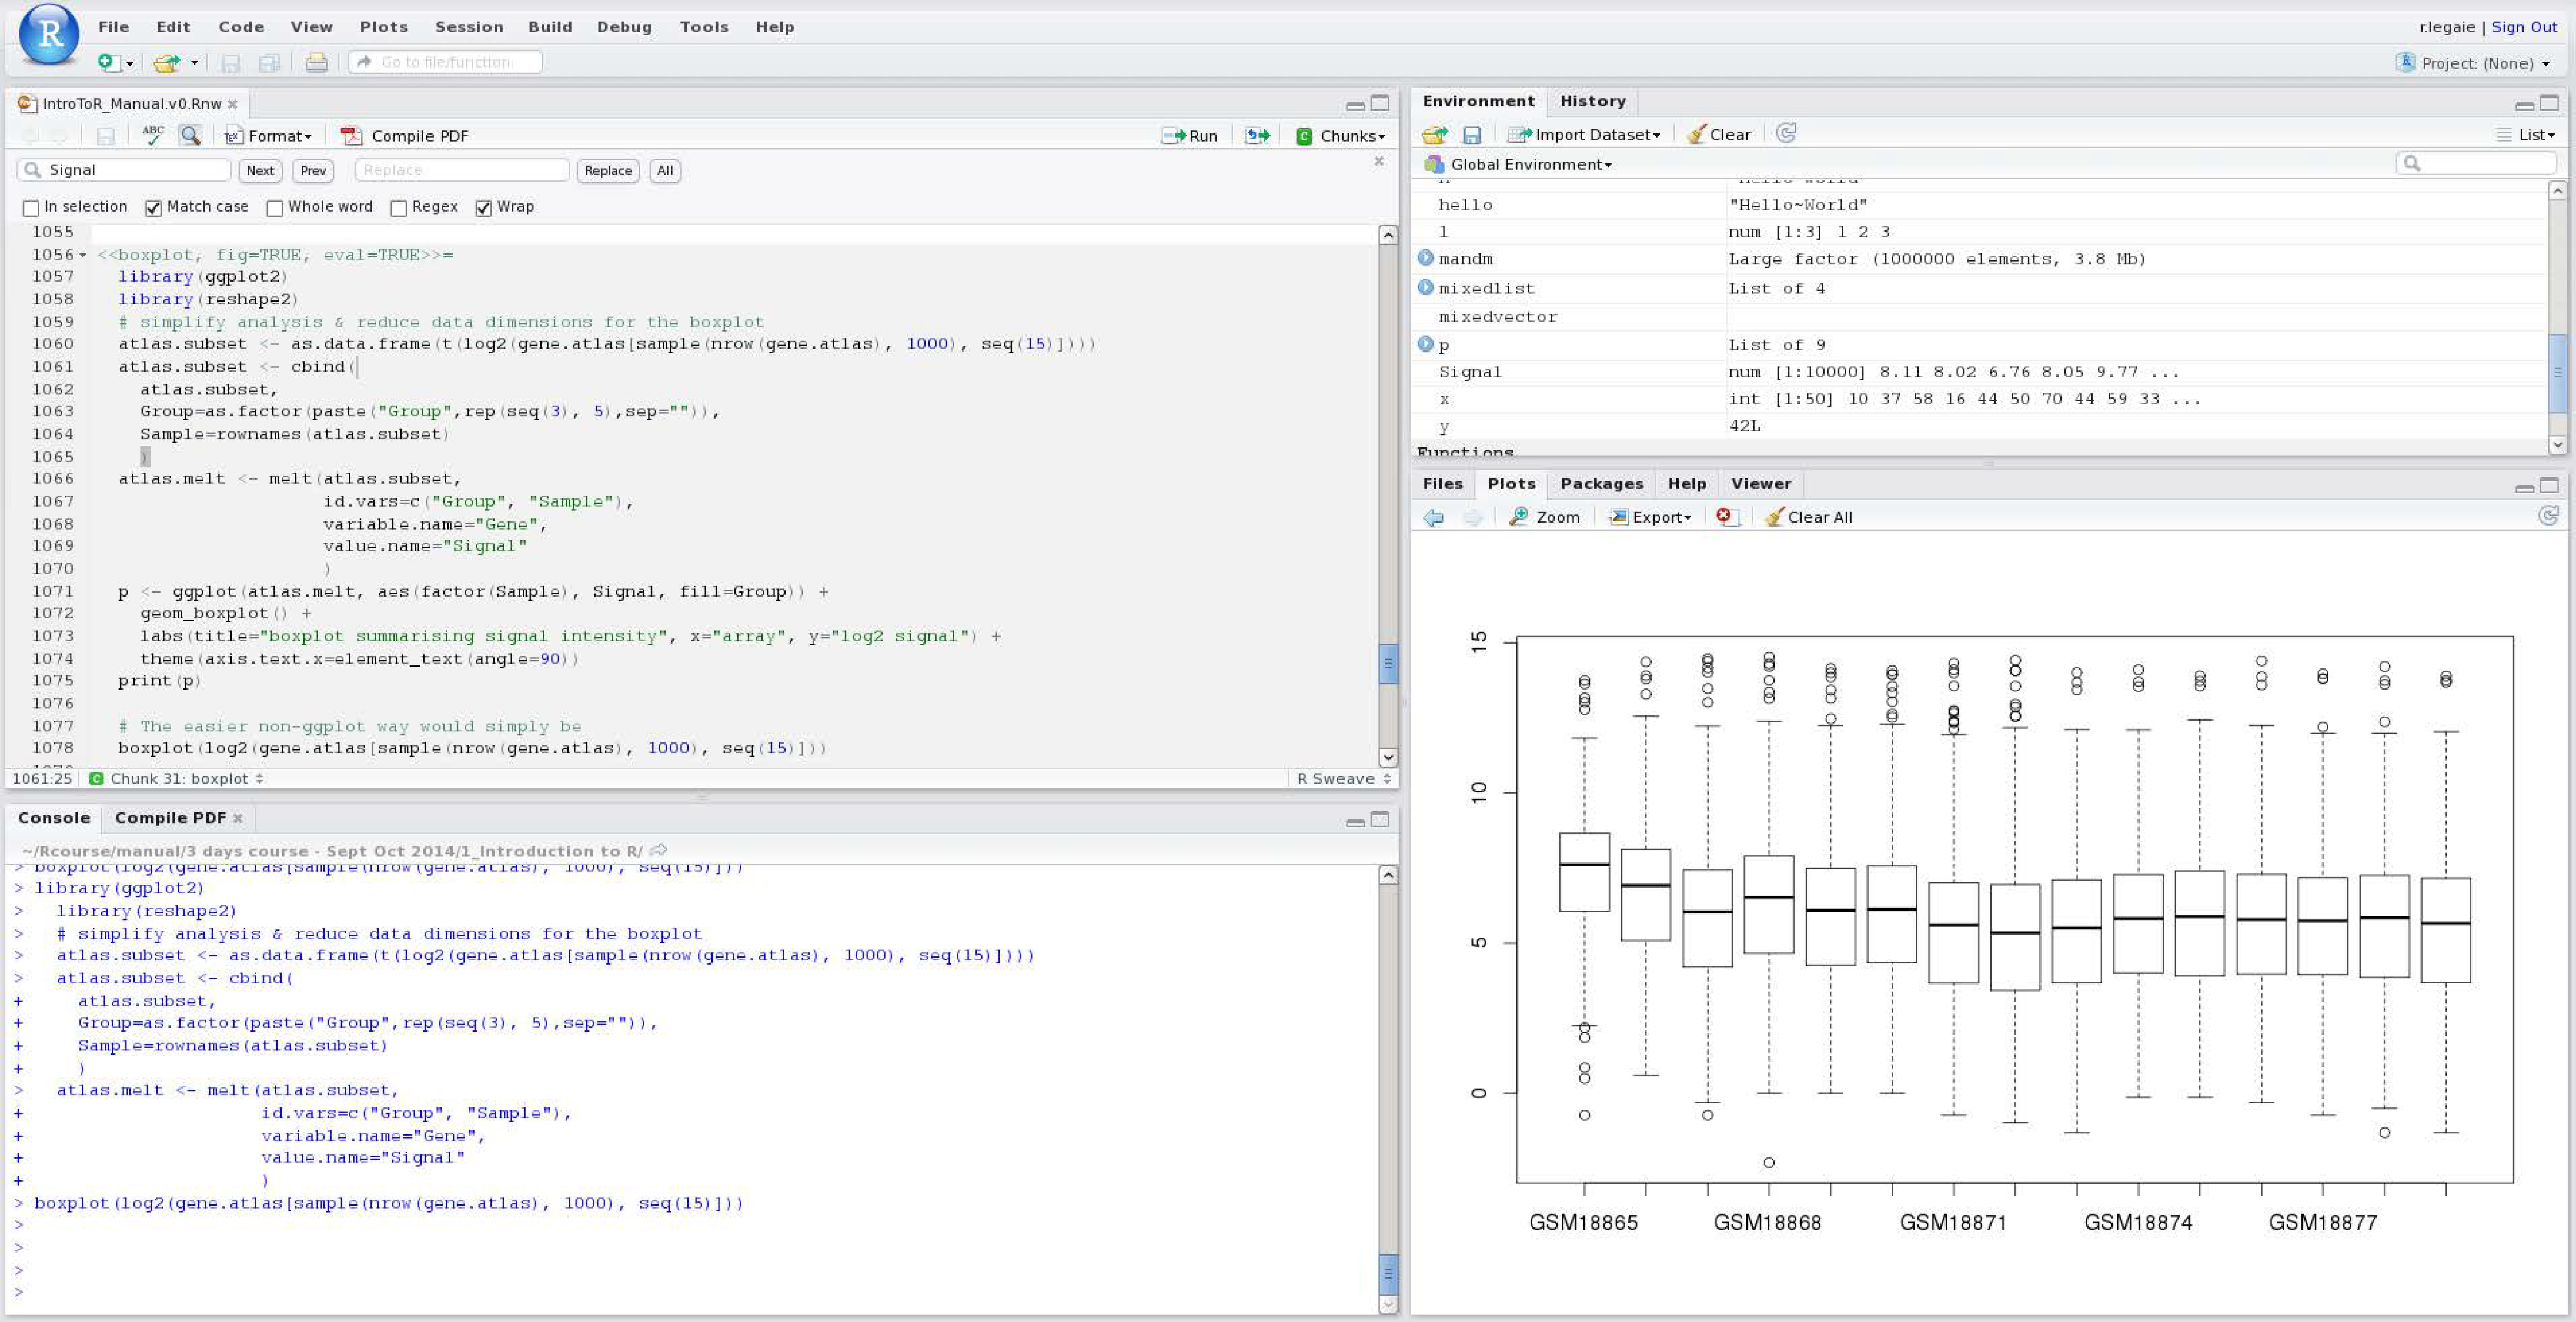
\includegraphics{images/RStudio-ide.png}
\caption{\label{fig:rstudio-ide}A screenshot of the RStudio session used in
the preparation of this course material. The document being prepared is
displayed in the top left pane. A figure is shown in the bottom right
pane and the loaded environment variables are presented in the top
right. Having access to all of these information in a single application
is simpler than managing an active R console, a text editor and an image
viewer.}
\end{figure}

RStudio integrates very cleanly with a number of best scientific working
practices (data sharing, reproducible research and research
documentation). RStudio allows for experiments to be performed in
projects - this allows you to create a separate workspace for each study
that you are performing. Code can be shared between projects easily and
Version Control (Subversion and Github) facilitate the sharing of
workflows and methods with other researchers.

For this course we recommend that you use our server version that has
been preconfigured for the software, packages and data that will be
used.

\begin{rmdexercise}
\textbf{Open up an RStudio server client and create a project}

\begin{enumerate}
\def\labelenumi{\arabic{enumi}.}
\item
  Open a web browser (not Internet Explorer) and connect to the server
  given to you by the trainer. Use the username and password that we
  have provided to connect and explore the options available in the top
  bar.
\item
  Explore the interface

  \begin{enumerate}
  \def\labelenumii{\alph{enumii})}
  \tightlist
  \item
    Where is the \textbf{Files} tab? What does it show? Can you see the
    \textbf{data} folder?
  \item
    Click the \textbf{data} folder to look inside, keep going until you
    get to some files
  \end{enumerate}
\item
  Click on the \textbf{Packages} tab and look at the list of packages
  that are installed in R. If you are ahead, scroll down and click on
  the \emph{methods} name. This should bring you to the \textbf{Help}
  tab, see what additional functions you can do using this package.

  \begin{itemize}
  \tightlist
  \item
    We will talk about what packages are later in the workshop.
  \end{itemize}

  \begin{enumerate}
  \def\labelenumii{\alph{enumii})}
  \tightlist
  \item
    In the top-right corner of the \textbf{Help} tab is a search text
    field. Type in \emph{``print''} and hit enter (if the autofinish
    starts to pop up click on print). This will show you the
    \texttt{print()} function and what parameters it accepts.
  \end{enumerate}
\end{enumerate}
\end{rmdexercise}

\section{Alternatives to RStudio}\label{alternatives-to-rstudio}

RStudio is not the only way to access R. The standard R installation
from CRAN (Comprehensive R Archive Network) provides a basic R graphical
user interface called the \textbf{R console}. This provides access to
the key R functionality and provides interfaces for the preparation of R
scripts. The simplest way to access R is perhaps through the command
line. With a typical R installation simply typing \texttt{"R"} at the
console should load an R session which you can directly interact with,
as seen in Figure \ref{fig:r-console}.

\begin{figure}[htbp]
\centering
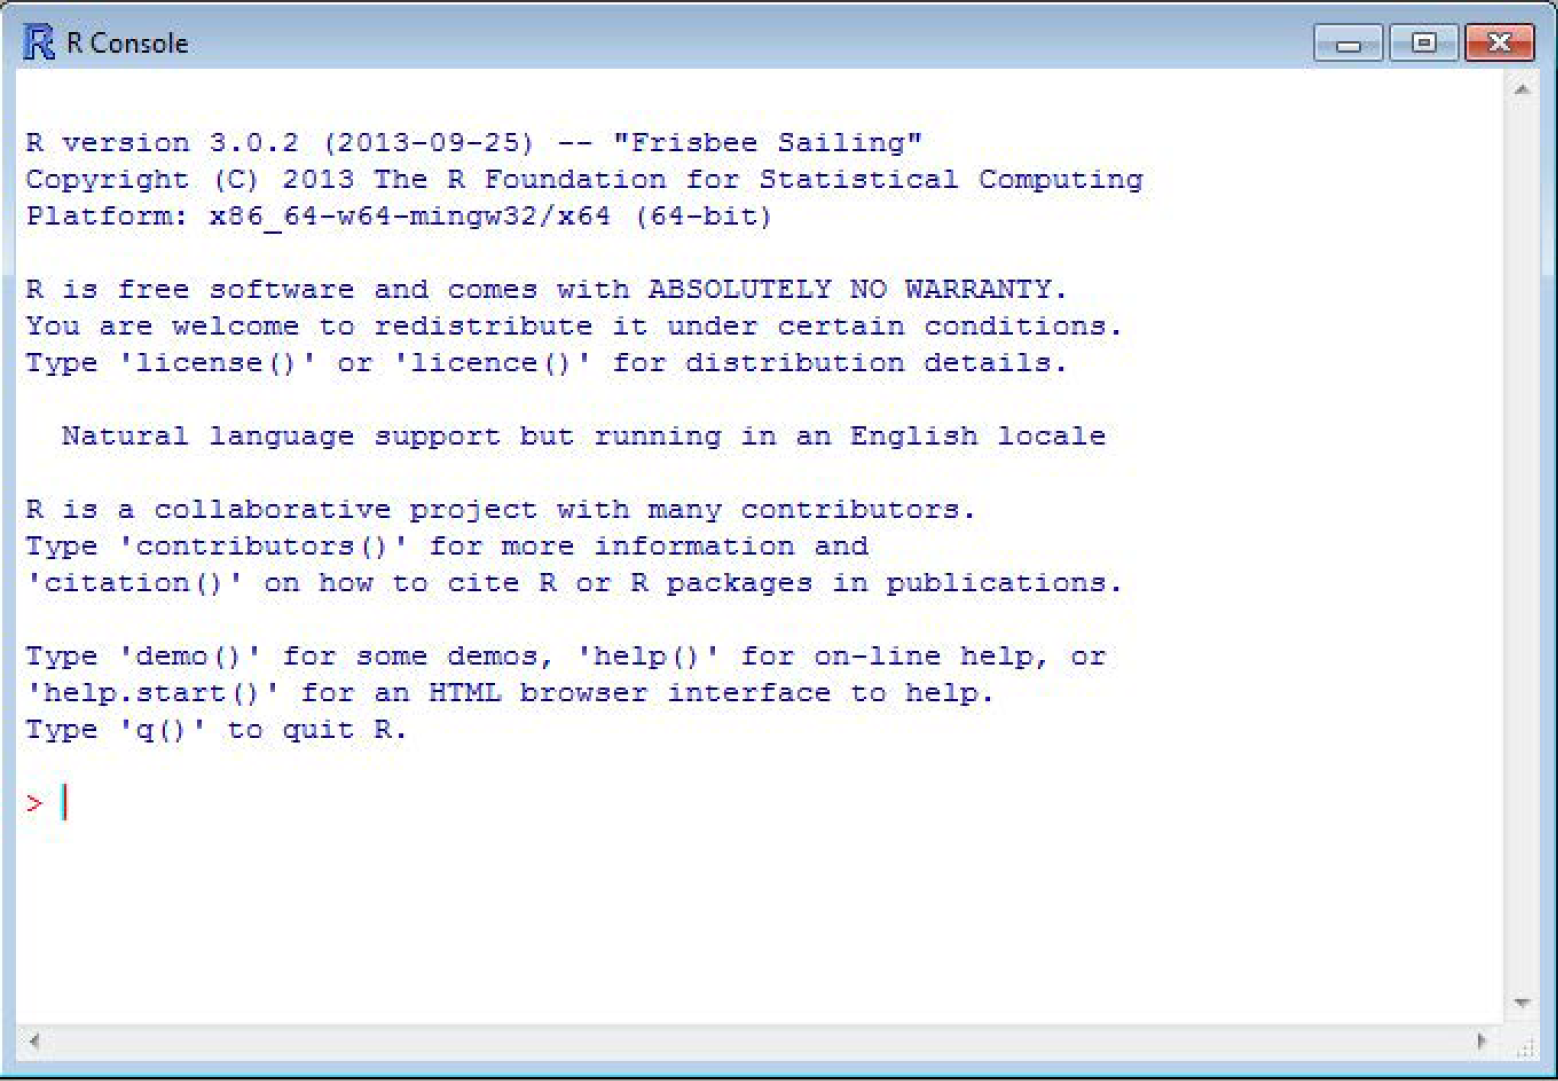
\includegraphics{images/R-console.png}
\caption{\label{fig:r-console}R installations typically include a basic R
editor and console that provide a basic framework for interacting with
the software, preparing R scripts and for the installation and
management of packages. This figure shows the R console as installed by
default on a Mac computer.}
\end{figure}

\section{The R workspace}\label{the-r-workspace}

The \textbf{workspace} refers to a R working environment and the
collection of data objects that have been created by the user. A
\textbf{session} refers to an instance of a workspace. In a session you
populate your workspace with a collection of objects and functions. A
session can be saved, this means that you can save the workspace content
so that the next time that you use R you can have all of the information
loaded and already available.

Session and workspace concepts are best understood within an environment
such as RStudio.

\section{Literate programming and
Reports}\label{literate-programming-and-reports}

\subsection{Literate programming}\label{literate-programming}

One of the most important things in scientific data analysis is to keep
a record of what analyses have been performed on data, why those
analyses were chosen, what settings were used, and what the output was.
Sometimes it is also necessary to write reports and summarise research
data to convince our supervisors, peers and students that we have a
solid handle on our science. Not only can R aid in the analysis of data
but it can also keep these records and/or write the research report for
you at the same time. There are a couple of different ways through which
this can be managed, and RStudio provides a number of simple ways to
automate the process of running R code, collecting the results of the
analysis and preparing a report in HTML or PDF format.

\begin{rmdexercise}
\textbf{Literate programming}

\begin{enumerate}
\def\labelenumi{\arabic{enumi}.}
\item
  Try some basic functions in the \textbf{Console} window (the large
  panel to the left)

  \begin{enumerate}
  \def\labelenumii{\alph{enumii})}
  \tightlist
  \item
    Type \texttt{1\ +\ 1} and hit enter, what is the output and where is
    it shown?
  \item
    Type \texttt{print("HELLO\ WORLD")} command in the console and hit
    hit.
  \item
    Try some other functions, e.g.: \texttt{3\^{}2} which is three
    squared or \texttt{11\%\%2} is the modulo function (the remainder
    left after the first number is divided by the second).
  \end{enumerate}
\item
  Now go to \textbf{File} menu and select \textbf{New File}
  \textgreater{} \textbf{R Script} and type the same commands in the
  \textbf{editor} window.

  \begin{enumerate}
  \def\labelenumii{\alph{enumii})}
  \tightlist
  \item
    highlight line {[}1{]} and click on the \textbf{Run} button at the
    top right of the editor window (or hit
    \textbf{{[}Ctrl{]}+{[}Enter{]}} on the keyboard)
  \item
    where is the output shown?
  \item
    highlight all three lines and click on the \textbf{Run} or
    \textbf{{[}Ctrl{]}+{[}Enter{]}}
  \end{enumerate}
\item
  Create a New Project that we will use for this course.

  \begin{enumerate}
  \def\labelenumii{\alph{enumii})}
  \tightlist
  \item
    Under the \textbf{File} menu, select \textbf{New Project}
  \item
    Click on \textbf{New Directory}, then \textbf{Empty Project}
  \item
    Select a name for your project. Generally this should reflect the
    analysis that you will be performing. Remember, you may want to come
    back to your projects months or even years in the future.
  \item
    You should now see an \texttt{.Rproj} file in your \textbf{Files}
    tab, with the name of the project you have just chosen. This file
    will contain your R session.
  \end{enumerate}
\end{enumerate}
\end{rmdexercise}

\subsection{KnitR}\label{knitr}

KnitR is a recent framework addition to the RStudio environment and one
that we encourage you to use as the basis for this workshop. KnitR is a
Markdown language that allows us to combine free text and R code into a
single document, and automatically generate documents that include both
these and the outputs of the R code. To start, let's open a new document
in RStudio of type \textbf{RMarkdown}. We will create a document and
discover how great R markdown is.

\begin{rmdexercise}
\textbf{Create a new knitR document}

\begin{enumerate}
\def\labelenumi{\arabic{enumi}.}
\item
  Under the \textbf{File} menu select \textbf{New File} \textgreater{}
  \textbf{R Markdown}. A window will appear in the top left of your
  RStudio interface containing your markdown code
\item
  Click on the question mark character and select \textbf{Markdown Quick
  Reference} for an guide to knitR formatting. This opens up in the
  \emph{Help} tab on the bottom-right window.
\item
  Change some of the free text that are denoted by the \emph{white
  background}.

  \begin{itemize}
  \tightlist
  \item
    The white free text sections contains subject titles and
    descriptions that will be included in your output document directly
    as they are written.
  \end{itemize}

  \begin{enumerate}
  \def\labelenumii{\alph{enumii})}
  \tightlist
  \item
    Replace line {[}1{]} 'Title' with something more meaningful.
  \item
    Save the file.
  \item
    Click on the \textbf{Knit HTML} button next to the question mark.
    You should see your rendered report in a new browser.

    \begin{itemize}
    \tightlist
    \item
      If a popup appears, click on ``Try again''.
    \end{itemize}
  \end{enumerate}
\item
  On a new line in the grey blocks, include one of the numerical
  calculations that you tried before. You can include multiple
  calculations if you like, but each one should be on a new line.
\item
  Click on \textbf{Knit HTML} to run your R code and produce an HTML
  format output of your knitR code
\end{enumerate}
\end{rmdexercise}

The white sections of an R Markdown document is the descriptive part of
your report. The grey blocks are referred to as \textbf{chunks} and
consists of \texttt{R\ code} that will be evaluated at run time and the
results included in the generated document. Chunks must following the
following syntax:

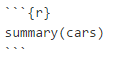
\includegraphics{images/Rchunk.png}

The \textbf{backquote} or \textbf{backtick} (`) character is the one
immediately to the left of `1' on your keyboard.

\begin{rmdtip}
\textbf{Using knitR}

\begin{itemize}
\tightlist
\item
  Save your knitR document regularly, to protect your code again the
  possibility of the software crashing. It will also be saved
  automatically when you click \textbf{Knit HTML}
\item
  Create a separate \emph{chunk} (or code block) for each subsection of
  the analysis. This makes troubleshooting and bug fixing much simpler.
\item
  You can run a \emph{chunk} (or code block) on its own by putting the
  cursor anywhere in that block and selecting \textbf{Chunks}
  \textgreater{} \textbf{Run Current Chunk} (top right of knitR window).
  Or you can run a single line by putting the cursor in that line and
  clicking the \textbf{Run} button (next to \textbf{Chunks})
\end{itemize}
\end{rmdtip}

\chapter{Data objects (variables) in
R}\label{data-objects-variables-in-r}

As with all other computer languages information needs to be stored in a
way that can be recalled, displayed and analysed. A variable name is
used to point to a data object in memory (or on disk).

A variable name should not start with a number, should not contain
spaces and should not contain special characters such as \#, \%, \&.
These characters require special handling and often lead to errors that
require debugging.

\section{Declaring objects}\label{declaring-objects}

Declaring a object (or variable) is simple in R, we just need to give it
a name and the content for that object. This can be done either directly
in the console or in a chunk if using knitR.

Remember that code entered into the console window will be executed
immediately when you press the {[}Enter{]} key. But do not expect output
for every line you enter, many R commands do not print anything to the
screen. Code in the knitR document will only be executed when you run
the chunk or click on \textbf{knit HTML}

\begin{rmdexercise}
\textbf{Declare an object}

\begin{enumerate}
\def\labelenumi{\arabic{enumi}.}
\item
  Enter the example code below into your RStudio interface. You can type
  it directly into the console and pressing the \textbf{{[}Enter{]} key}
  after each line or create a new chunk in your knitR document for all
  lines.

  \begin{enumerate}
  \def\labelenumii{\alph{enumii})}
  \tightlist
  \item
    Did you get any output after executing line {[}1{]}?
  \end{enumerate}
\item
  If you entered above code in the console, click on the
  \textbf{Environment} tab in the top-right corner window. Do you see
  the value \texttt{x} listed? If you do not then try again (or select
  the \texttt{x\ \textless{}-\ 42} line in your knitR and click on
  \textbf{Run}).

  \begin{enumerate}
  \def\labelenumii{\alph{enumii})}
  \tightlist
  \item
    Try other commands, e.g. \texttt{y\ \textless{}-\ 555}, do you see a
    new variable \texttt{y} listed in the \emph{Environment} tab?
  \end{enumerate}
\end{enumerate}
\end{rmdexercise}

\begin{Shaded}
\begin{Highlighting}[]
\NormalTok{x <-}\StringTok{ }\DecValTok{42}

\CommentTok{# this has set x to the value of 42}
\NormalTok{x}
\end{Highlighting}
\end{Shaded}

\begin{verbatim}
## [1] 42
\end{verbatim}

\begin{Shaded}
\begin{Highlighting}[]
\KeywordTok{print}\NormalTok{(x)}
\end{Highlighting}
\end{Shaded}

\begin{verbatim}
## [1] 42
\end{verbatim}

\textbf{Setting object values and viewing object contents}

\begin{longtable}[]{@{}ll@{}}
\toprule
\begin{minipage}[b]{0.13\columnwidth}\raggedright\strut
Command\strut
\end{minipage} & \begin{minipage}[b]{0.81\columnwidth}\raggedright\strut
Description\strut
\end{minipage}\tabularnewline
\midrule
\endhead
\begin{minipage}[t]{0.13\columnwidth}\raggedright\strut
\texttt{\textless{}-}\strut
\end{minipage} & \begin{minipage}[t]{0.81\columnwidth}\raggedright\strut
This marker is used to set an object's value. The more standard
\texttt{=} operator will also work but they have different levels of
precedence. As best practice it is better to use
\texttt{\textless{}-}.\strut
\end{minipage}\tabularnewline
\begin{minipage}[t]{0.13\columnwidth}\raggedright\strut
\texttt{\#}\strut
\end{minipage} & \begin{minipage}[t]{0.81\columnwidth}\raggedright\strut
The hashmark at the start of line is a way to comment your code. This
directs R to ignore the rest of the current line. Commenting your good
is very good practice and is also used lots to remove commands that you
may use in debugging a more complex workflow.\strut
\end{minipage}\tabularnewline
\begin{minipage}[t]{0.13\columnwidth}\raggedright\strut
\texttt{print()}\strut
\end{minipage} & \begin{minipage}[t]{0.81\columnwidth}\raggedright\strut
Is the print function which writes out the value of the object. Simply
typing the name of the object will also write out the value contained
with in as seen in the examples above: \texttt{x} and
\texttt{print(x)}\strut
\end{minipage}\tabularnewline
\bottomrule
\end{longtable}

\begin{rmdtip}
\textbf{KnitR and Console workspaces}

\begin{itemize}
\tightlist
\item
  It is important to remember that \textbf{knitR} and the
  \textbf{Console} window operate in different workspaces. This means
  that if you declare a object in your knitR code and then \textbf{knit
  HTML}, that object will not be available within the console. In the
  exercise above, if you created the code as a knitR chunk and then ran
  \textbf{knit HTML}, try now entering \texttt{print(x)} into the
  console box. You should get an error
  \texttt{Error:\ object\ x\ not\ found} because \texttt{x} was only
  created within the knitR workspace. Conversely, \textbf{knit HTML}
  cannot access any objects that were created only in your
  \textbf{Console} window.
\item
  Also remember that when you use the \textbf{Run} or \textbf{Run chunk}
  options, that command will be run and objects created in the Console
  session, not in the knitR session.
\end{itemize}
\end{rmdtip}

\section{Datatypes}\label{datatypes}

In common with many computer languages, every object in R is assigned a
\textbf{type}. The primary data types in R are Numeric, Integer,
Character, Logical, and Complex (which is used for specialist
mathematical applications). The type of an object determines what data
can be stored within it and often, what functions can be applied to it.

\subsection{Numeric}\label{numeric}

Decimal values are called \textbf{numerics} in R. In the previous
section we declared an object called \texttt{x}, to which we assigned
the value of 42. R recognised this as a number and automatically set the
type of \texttt{x} to be numeric. We can test whether an object is a
numeric using the \texttt{is.numeric()} function. Or, we can ask
directly what type it is using \texttt{class()}.

\begin{Shaded}
\begin{Highlighting}[]
\KeywordTok{is.numeric}\NormalTok{(x)}
\end{Highlighting}
\end{Shaded}

\begin{verbatim}
## [1] TRUE
\end{verbatim}

\begin{Shaded}
\begin{Highlighting}[]
\KeywordTok{class}\NormalTok{(x)}
\end{Highlighting}
\end{Shaded}

\begin{verbatim}
## [1] "numeric"
\end{verbatim}

\subsection{Integer}\label{integer}

\textbf{Integers} are a separate type to numerics and contain
\emph{whole number} values only. Just as we can test whether an object
is a numeric, we can also test whether one is an integer:

\begin{Shaded}
\begin{Highlighting}[]
\KeywordTok{is.integer}\NormalTok{(x)}
\end{Highlighting}
\end{Shaded}

\begin{verbatim}
## [1] FALSE
\end{verbatim}

Strangely, although 42 is indeed an integer, this reports \(FALSE\).
This is because \texttt{x} has been \textbf{cast} as a numeric and an
object can only be of a single type. Indeed even \texttt{is.integer(42)}
returns \(FALSE\) because R by default assigns any numerical value as
type numeric.

\subsubsection{Typecasting}\label{typecasting}

If we want to perform integer functions on \texttt{x}, we can force it
from one type to another, in this case using the \texttt{as.integer()}
function. This is known as \textbf{typecasting}. The
\texttt{as.integer()} function also forces non-whole numbers into
integers by rounding them down to the nearest whole number.

\begin{Shaded}
\begin{Highlighting}[]
\NormalTok{y <-}\StringTok{ }\KeywordTok{as.integer}\NormalTok{(x)}
\KeywordTok{is.integer}\NormalTok{(y)}
\end{Highlighting}
\end{Shaded}

\begin{verbatim}
## [1] TRUE
\end{verbatim}

\begin{Shaded}
\begin{Highlighting}[]
\KeywordTok{class}\NormalTok{(y)}
\end{Highlighting}
\end{Shaded}

\begin{verbatim}
## [1] "integer"
\end{verbatim}

\begin{Shaded}
\begin{Highlighting}[]
\KeywordTok{as.integer}\NormalTok{(}\FloatTok{3.1415}\NormalTok{)}
\end{Highlighting}
\end{Shaded}

\begin{verbatim}
## [1] 3
\end{verbatim}

\begin{rmdtip}
\textbf{Writing to objects or the screen}

\begin{itemize}
\item
  In the example above, you will notice that the line
  \texttt{y\ \textless{}-\ as.integer(x)} generates no output, while
  \texttt{as.integer(3.1415)} prints a result to screen. This is because
  in the first case, the output of \texttt{as.integer} is passed into
  the object \texttt{y}, while in the second case, no destination is
  given so by default it prints to screen.
\item
  This also means that the output from the first command can be accessed
  and used again later by calling \texttt{y} but the output from the
  second is lost and cannot be used by future R commands.
\end{itemize}
\end{rmdtip}

\subsection{Logical}\label{logical}

\textbf{Logical} datatypes can have one of only two values:
\texttt{TRUE} or \texttt{FALSE}. \textbf{Note}, these are case-specific,
\texttt{True} or \texttt{true} are not valid logical values. However,
the shortcut: \texttt{T} and \texttt{F} will work.

\begin{Shaded}
\begin{Highlighting}[]
\OtherTok{TRUE}
\end{Highlighting}
\end{Shaded}

\begin{verbatim}
## [1] TRUE
\end{verbatim}

\begin{Shaded}
\begin{Highlighting}[]
\OtherTok{TRUE} \NormalTok{==}\StringTok{ }\OtherTok{TRUE}
\end{Highlighting}
\end{Shaded}

\begin{verbatim}
## [1] TRUE
\end{verbatim}

\begin{Shaded}
\begin{Highlighting}[]
\OtherTok{TRUE} \NormalTok{==}\StringTok{ }\OtherTok{FALSE}
\end{Highlighting}
\end{Shaded}

\begin{verbatim}
## [1] FALSE
\end{verbatim}

\begin{Shaded}
\begin{Highlighting}[]
\OtherTok{TRUE} \NormalTok{!=}\StringTok{ }\OtherTok{FALSE}
\end{Highlighting}
\end{Shaded}

\begin{verbatim}
## [1] TRUE
\end{verbatim}

\begin{Shaded}
\begin{Highlighting}[]
\KeywordTok{class}\NormalTok{(}\OtherTok{FALSE}\NormalTok{)}
\end{Highlighting}
\end{Shaded}

\begin{verbatim}
## [1] "logical"
\end{verbatim}

\begin{Shaded}
\begin{Highlighting}[]
\CommentTok{# Logicals can also be typecast}
\KeywordTok{as.integer}\NormalTok{(}\OtherTok{TRUE}\NormalTok{)}
\end{Highlighting}
\end{Shaded}

\begin{verbatim}
## [1] 1
\end{verbatim}

\begin{rmdexercise}
\begin{enumerate}
\def\labelenumi{\arabic{enumi}.}
\item
  Now try typecasting \texttt{FALSE} to an integer.
\item
  Next try typecasting in the reverse, that is, converting the digits
  (1, 0) into TRUE or FALSE. \emph{Hint}: \texttt{as.logical()}
\item
  {[}\textbf{Optional}{]} If you are ahead, have a look at typecasting
  other values (e.g. \textgreater{}1 and \textless{}0) into logical
  types. Can you see what is happening?
\end{enumerate}
\end{rmdexercise}

\subsection{Character}\label{character}

A \textbf{character} object is used to represent strings or text values
in R. We convert objects into character values with the
\texttt{as.character()} function:

\begin{Shaded}
\begin{Highlighting}[]
\NormalTok{h <-}\StringTok{ "Hello world"}
\KeywordTok{class}\NormalTok{(h)}
\end{Highlighting}
\end{Shaded}

\begin{verbatim}
## [1] "character"
\end{verbatim}

\begin{Shaded}
\begin{Highlighting}[]
\KeywordTok{as.character}\NormalTok{(x)}
\end{Highlighting}
\end{Shaded}

\begin{verbatim}
## [1] "42"
\end{verbatim}

\begin{Shaded}
\begin{Highlighting}[]
\KeywordTok{as.character}\NormalTok{(}\OtherTok{FALSE}\NormalTok{)}
\end{Highlighting}
\end{Shaded}

\begin{verbatim}
## [1] "FALSE"
\end{verbatim}

\begin{rmdexercise}
\textbf{Setting, retrieving and changing data types}

\begin{enumerate}
\def\labelenumi{\arabic{enumi}.}
\item
  Enter the code blocks from the sections above (from Numerics through
  to Character) into your RStudio interface (as before, either into the
  console or the knitR document), and run them to generate the output.

  \begin{itemize}
  \tightlist
  \item
    Remember, you can use the \emph{Environments} tab to keep a track of
    the objects being created.
  \item
    \textbf{Note}, below all the outputs are shown altogether for
    readability. If you are running them in console, you will see the
    output immediately as you hit {[}Enter{]}.
  \end{itemize}
\item
  Experiment with different values so you understand better how the
  types and typecasting behave.
\item
  Characters are much more interesting than just storing a piece of
  text. Try the commands below, which explore a number of fundamental
  character manipulating functions explained further below.
\end{enumerate}
\end{rmdexercise}

\begin{Shaded}
\begin{Highlighting}[]
\NormalTok{letters <-}\StringTok{ }\KeywordTok{c}\NormalTok{(}\StringTok{"A"}\NormalTok{, }\StringTok{"B"}\NormalTok{, }\StringTok{"C"}\NormalTok{)}
\KeywordTok{paste}\NormalTok{(letters, }\DataTypeTok{collapse=}\StringTok{" "}\NormalTok{)}
\NormalTok{hello <-}\StringTok{ }\KeywordTok{paste}\NormalTok{(}\StringTok{"Hello"}\NormalTok{, }\StringTok{"World"}\NormalTok{, }\DataTypeTok{sep=}\StringTok{"~"}\NormalTok{)}
\KeywordTok{nchar}\NormalTok{(hello)}
\KeywordTok{substr}\NormalTok{(hello, }\KeywordTok{which}\NormalTok{(}\KeywordTok{strsplit}\NormalTok{(hello, }\StringTok{''}\NormalTok{)[[}\DecValTok{1}\NormalTok{]]==}\StringTok{'~'}\NormalTok{)+}\DecValTok{1}\NormalTok{, }\KeywordTok{nchar}\NormalTok{(hello))}

\KeywordTok{gsub}\NormalTok{(}\StringTok{"World"}\NormalTok{, }\StringTok{"R"}\NormalTok{, hello)}
\KeywordTok{grep}\NormalTok{(}\StringTok{"Hello"}\NormalTok{, hello)}
\KeywordTok{grepl}\NormalTok{(}\StringTok{"Stephen"}\NormalTok{, hello)}
\end{Highlighting}
\end{Shaded}

\begin{verbatim}
## [1] "A B C"
## [1] 11
## [1] "World"
## [1] "Hello~R"
## [1] 1
## [1] FALSE
\end{verbatim}

\textbf{Characters, strings and regular expressions}

\begin{longtable}[]{@{}ll@{}}
\toprule
\begin{minipage}[b]{0.21\columnwidth}\raggedright\strut
Function\strut
\end{minipage} & \begin{minipage}[b]{0.73\columnwidth}\raggedright\strut
Description\strut
\end{minipage}\tabularnewline
\midrule
\endhead
\begin{minipage}[t]{0.21\columnwidth}\raggedright\strut
\texttt{paste()}\strut
\end{minipage} & \begin{minipage}[t]{0.73\columnwidth}\raggedright\strut
is used to concatenate two or more character objects into a single
object. The concatenation can be performed on an object which is itself
a list, vector or factor or can be run using individually specified
character objects. The sep and collapse arguments are used to specify
the delimiter that will be used to link the objects together.\strut
\end{minipage}\tabularnewline
\begin{minipage}[t]{0.21\columnwidth}\raggedright\strut
\texttt{nchar()}\strut
\end{minipage} & \begin{minipage}[t]{0.73\columnwidth}\raggedright\strut
returns an integer value that corresponds to the number of characters
contained within the object.\strut
\end{minipage}\tabularnewline
\begin{minipage}[t]{0.21\columnwidth}\raggedright\strut
\texttt{substr()}\strut
\end{minipage} & \begin{minipage}[t]{0.73\columnwidth}\raggedright\strut
is used to prepare a substring from a character object using the start
and stop coordinates of the substring to retain. The \texttt{substr}
command provided uses slicing of a list object, this will be introduced
further in Section {[}data-structures{]}\strut
\end{minipage}\tabularnewline
\begin{minipage}[t]{0.21\columnwidth}\raggedright\strut
\texttt{strsplit()}\strut
\end{minipage} & \begin{minipage}[t]{0.73\columnwidth}\raggedright\strut
splits a character object into a list of character objects based on a
delimiter. If an empty delimiter argument is provided the individual
characters will be returned.\strut
\end{minipage}\tabularnewline
\begin{minipage}[t]{0.21\columnwidth}\raggedright\strut
\texttt{gsub()}\strut
\end{minipage} & \begin{minipage}[t]{0.73\columnwidth}\raggedright\strut
is used to substitute a substring in the given character object with a
different (or empty) substring.\strut
\end{minipage}\tabularnewline
\begin{minipage}[t]{0.21\columnwidth}\raggedright\strut
\texttt{grep()}\strut
\end{minipage} & \begin{minipage}[t]{0.73\columnwidth}\raggedright\strut
may be used to identify which elements of a vector contain a given
substring character query while grepl() provides a vector of logical
responses as to whether the substring exists in each element.\strut
\end{minipage}\tabularnewline
\bottomrule
\end{longtable}

\section{Functions}\label{functions}

Before we move onto data structures in the next section, we will take an
aside to look at \textbf{functions}. Functions are a group of commands
that perform a specific action. By itself it is not a complete
executable program but form part of a larger workflow. Like variables
that hold data, functions are also given a name so that they can be
\emph{reused}. They generally follow the
\texttt{input\ -\textgreater{}\ process\ -\textgreater{}\ output} model,
that is, they take input, do something with the input and produce
output. The output can either be printed to the screen or be
\emph{returned} and assigned to a variable that holds the new data.

So far we have already started using some of the in-build functions in R
like \texttt{print()}, \texttt{str()}, \texttt{as.integer()} etc. They
take the form of
\texttt{output\_variable\ \textless{}-\ function\_name(input\_variable)}
where the output\_variable is optional.

Other than assigning the output of a function to a variable, functions
can also be \textbf{nested} within other functions. For example, in the
previous exercise, there was the line:

\begin{Shaded}
\begin{Highlighting}[]
\NormalTok{letters <-}\StringTok{ }\KeywordTok{c}\NormalTok{(}\StringTok{"A"}\NormalTok{,}\StringTok{"B"}\NormalTok{,}\StringTok{"C"}\NormalTok{)}
\KeywordTok{paste}\NormalTok{(letters, }\DataTypeTok{collapse=}\StringTok{" "}\NormalTok{)}
\end{Highlighting}
\end{Shaded}

Since the object \texttt{letters} is not going to be used anywhere else
in our program, we can simply nest the two lines together such that:

\begin{Shaded}
\begin{Highlighting}[]
\KeywordTok{paste}\NormalTok{(}\KeywordTok{c}\NormalTok{(}\StringTok{"A"}\NormalTok{,}\StringTok{"B"}\NormalTok{,}\StringTok{"C"}\NormalTok{))}
\end{Highlighting}
\end{Shaded}

Just like in mathematics, the \textbf{order of operations} (or
\emph{operator precedence}) is the same in R. Operations are evaluated
(or executed) from the innermost brackets first. So in the command
above, the inner \texttt{c("A","B","C")} is executed first and the
output (which is held temporarily in memory) is then passed to the outer
function \texttt{paste()}.

With this shortcut, you can reduce the resources that a program takes
(not to mention the lines of code) and create very complex nested
function calls. Keep an eye out for nested functions throughout the
workshop.

\begin{rmdtip}
When new to R and coming across a complex nested function call, the tip
is to \textbf{break it up} into sections. Break the functions into
smaller pieces \emph{starting from the innermost function} and assign
them to variables first. Execute each line, one at a time and examine
the output. Then when you are comfortable with waht each line is doing,
put the pieces together again. This will help you understand what each
function is doing first before trying to decipher the entire line in one
go. Once you become familiar with more functions, reading nested
functions will become a breeze!
\end{rmdtip}

\section{Data structures}\label{data-structures}

We do not typically expect to work with atomic objects during an
\emph{-omics} analysis. To make the best use of R we want to use
hundreds, thousands and millions of data points. We arrange these in one
of a number of different data structures: vectors, lists, matrices and
data frames.

\subsection{Vectors}\label{vectors}

A \textbf{vector} is a group of components of the \emph{same} type.
Elements of a vector can be accessed by their numeric position (referred
to as \textbf{indexing}) starting at position 1. They can also be named
so that we can access the object component using the namespace. The
\texttt{c()} function (for \emph{combine}) is used to join a number of
single values together into a vector.

\begin{Shaded}
\begin{Highlighting}[]
\NormalTok{l <-}\StringTok{ }\KeywordTok{c}\NormalTok{(}\DecValTok{1}\NormalTok{,}\DecValTok{2}\NormalTok{,}\DecValTok{3}\NormalTok{)}
\KeywordTok{is.vector}\NormalTok{(l)}
\end{Highlighting}
\end{Shaded}

\begin{verbatim}
## [1] TRUE
\end{verbatim}

Access the second element of the vector:

\begin{Shaded}
\begin{Highlighting}[]
\NormalTok{l[}\DecValTok{2}\NormalTok{]}
\end{Highlighting}
\end{Shaded}

\begin{verbatim}
## [1] 2
\end{verbatim}

What happens if we try to mix data types in a vector? \texttt{str()} is
a function that describes the structure of an object.

\begin{Shaded}
\begin{Highlighting}[]
\NormalTok{mixedVector <-}\StringTok{ }\KeywordTok{c}\NormalTok{(}\DataTypeTok{animal=}\StringTok{"sheep"}\NormalTok{, }\DataTypeTok{meaningOfLife=}\KeywordTok{as.integer}\NormalTok{(}\DecValTok{42}\NormalTok{), }\DataTypeTok{pi=}\FloatTok{3.1415}\NormalTok{)}
\KeywordTok{str}\NormalTok{(mixedVector)}
\end{Highlighting}
\end{Shaded}

\begin{verbatim}
##  Named chr [1:3] "sheep" "42" "3.1415"
##  - attr(*, "names")= chr [1:3] "animal" "meaningOfLife" "pi"
\end{verbatim}

\texttt{c()} can be used to combine vectors, not just individual values:

\begin{Shaded}
\begin{Highlighting}[]
\KeywordTok{c}\NormalTok{(l, mixedVector)}
\end{Highlighting}
\end{Shaded}

\begin{verbatim}
##                                                  animal meaningOfLife 
##           "1"           "2"           "3"       "sheep"          "42" 
##            pi 
##      "3.1415"
\end{verbatim}

\begin{rmdexercise}
\textbf{Using vectors}

\begin{enumerate}
\def\labelenumi{\arabic{enumi}.}
\item
  Enter the code block above into your RStudio interface and review the
  output.
\item
  Now enter the next code block below and review the output.

  \begin{enumerate}
  \def\labelenumii{\alph{enumii})}
  \tightlist
  \item
    Can you determine the difference between \texttt{mixedVector{[}2{]}}
    and \texttt{mixedVector{[}{[}2{]}{]}}?
  \end{enumerate}
\item
  What would the equivalent command to \texttt{mixedVector{[}{[}2{]}{]}}
  be if you were accessing the vector by name?
\end{enumerate}
\end{rmdexercise}

\begin{Shaded}
\begin{Highlighting}[]
\CommentTok{#Access some elements of mixedVector by position or name}
\NormalTok{mixedVector[}\DecValTok{2}\NormalTok{]}
\NormalTok{mixedVector[[}\DecValTok{2}\NormalTok{]]}
\NormalTok{mixedVector[}\StringTok{'animal'}\NormalTok{]}
\KeywordTok{names}\NormalTok{(mixedVector)}
\end{Highlighting}
\end{Shaded}

\begin{rmdtip}
\textbf{Vectors and Collections of data}

\begin{itemize}
\tightlist
\item
  Because elements of a vector must be the same type, when we
  investigate the content of \texttt{mixedVector} we can observe that
  the string, integer and numeric have all been cast to character.
\item
  \texttt{mixedVector} is a named vector, so we can access elements by
  name as well as position.
\end{itemize}
\end{rmdtip}

\subsection{Lists}\label{lists}

\textbf{Lists} are similar to vectors in that the are one-dimensional
structures for storing data, and like vectors can be accessed by
position or namespace. They differ from vectors in that they can contain
multiple \emph{different} data types. This makes them more flexible for
storing data but more limited in the analyses that can be performed on
them. Lists are created using the \texttt{list()} command, which has a
similar format to \texttt{c()}.

\begin{Shaded}
\begin{Highlighting}[]
\NormalTok{mixedList <-}\StringTok{ }\KeywordTok{list}\NormalTok{(}\DataTypeTok{animal=}\StringTok{"sheep"}\NormalTok{, }\DataTypeTok{meaningOfLife=}\KeywordTok{as.integer}\NormalTok{(}\DecValTok{42}\NormalTok{), }\DataTypeTok{pi=}\FloatTok{3.1415}\NormalTok{)}
\KeywordTok{str}\NormalTok{(mixedList)}
\end{Highlighting}
\end{Shaded}

\begin{verbatim}
## List of 3
##  $ animal       : chr "sheep"
##  $ meaningOfLife: int 42
##  $ pi           : num 3.14
\end{verbatim}

\begin{rmdtip}
\textbf{Checking for membership}

\begin{itemize}
\tightlist
\item
  \texttt{\%in\%} is a way to test the membership of a single element in
  a list or vector of items. For example, try typing in the command:
  \texttt{"sheep"\ \%in\%\ mixedList}
\end{itemize}
\end{rmdtip}

\subsection{Changing Vectors and
Lists}\label{changing-vectors-and-lists}

While a list or vector is useful, their utility is much greater when we
can add or remove elements from them, or change the value of existing
elements.

\begin{Shaded}
\begin{Highlighting}[]
\CommentTok{# Add an item named 'pens' with a numeric value of 3 to the list}
\NormalTok{mixedList <-}\StringTok{ }\KeywordTok{append}\NormalTok{(mixedList, }\KeywordTok{c}\NormalTok{(}\DataTypeTok{pens=}\DecValTok{3}\NormalTok{))}

\CommentTok{# Now add another item named 'papers' with a chr value of 'bioinformatics'}
\NormalTok{mixedList <-}\StringTok{ }\KeywordTok{append}\NormalTok{(mixedList, }\KeywordTok{c}\NormalTok{(}\DataTypeTok{papers=}\StringTok{"bioinformatics"}\NormalTok{))}

\CommentTok{# Display just the second element of the list}
\NormalTok{mixedList[}\DecValTok{2}\NormalTok{]}
\end{Highlighting}
\end{Shaded}

\begin{verbatim}
## $meaningOfLife
## [1] 42
\end{verbatim}

\begin{Shaded}
\begin{Highlighting}[]
\CommentTok{# Display all but the second element of the list}
\NormalTok{mixedList[-}\DecValTok{2}\NormalTok{]}
\end{Highlighting}
\end{Shaded}

\begin{verbatim}
## $animal
## [1] "sheep"
## 
## $pi
## [1] 3.1415
## 
## $pens
## [1] 3
## 
## $papers
## [1] "bioinformatics"
\end{verbatim}

\begin{Shaded}
\begin{Highlighting}[]
\CommentTok{# Change the value of the pens item}
\NormalTok{mixedList$pens <-}\StringTok{ }\DecValTok{4}

\CommentTok{# Remove the papers item}
\NormalTok{mixedList$papers <-}\StringTok{ }\OtherTok{NULL}
\end{Highlighting}
\end{Shaded}

\begin{rmdexercise}
\textbf{Using Lists}

\begin{enumerate}
\def\labelenumi{\arabic{enumi}.}
\item
  Enter the two \texttt{mixedList} code blocks into RStudio and review
  the output.
\item
  Try and retrieve different elements of the list

  \begin{enumerate}
  \def\labelenumii{\alph{enumii})}
  \tightlist
  \item
    Can you get the second \textbf{and} fourth elements? (\emph{Hint:}
    \texttt{c()})
  \item
    What about everything BUT the second \textbf{and} fourth?
  \end{enumerate}
\item
  {[}\textbf{Optional}{]} If you are ahead, now try to getting a range
  of values, that is get the third to the forth elements. \emph{Hint:}
  colon (:) symbol.
\end{enumerate}
\end{rmdexercise}

Now let us imagine that QFAB is actually performing a study on the
course participants. To perform subsequent statistical testing we will
need to know a little something about each of our consenting subjects,
and we are going to build a data structure to store this information.

\begin{rmdexercise}
\begin{enumerate}
\def\labelenumi{\arabic{enumi}.}
\setcounter{enumi}{2}
\item
  Create three vectors that contain, respectively, the names, sex and
  age of the research cohort on this course.

  \begin{itemize}
  \tightlist
  \item
    Let's have the vectors of type:

    \begin{itemize}
    \tightlist
    \item
      character for \texttt{name}
    \item
      logical for \texttt{sex} (e.g.~have female be TRUE) and
    \item
      integer for \texttt{age}
    \end{itemize}
  \end{itemize}

  \begin{enumerate}
  \def\labelenumii{\alph{enumii})}
  \tightlist
  \item
    When you have these vectors created, place them all in a single list
    called \texttt{subject}
  \end{enumerate}
\end{enumerate}
\end{rmdexercise}

\subsection{Factors}\label{factors}

\textbf{Factors} are vector objects that contain grouping
(classification) information of its components. Functionally they are
similar to vectors in that they are a collection of objects of a
\emph{single} type. Factors are best applied when there are a limited
number of different values. They are often used when categorical values
are used in modelling or presenting data, e.g.~phenotypic or study class
data, such as diabetic, pre-diabetic, healthy.

For the example that we explore in the following exercise, we are going
to consider a massive bucket of M\&Ms.~Assuming that the different
colours are randomly mixed with an equal probability we would like to
explore a million different sweets.

\begin{rmdexercise}
\textbf{Using Factors}

Use the code below to create a factorised \texttt{mandm} vector
containing 1 million M\&Ms of various colours.

\emph{Note}, the output is again grouped together at the end for
readability. The table below explains the new functions and what they
mean.
\end{rmdexercise}

\begin{Shaded}
\begin{Highlighting}[]
\NormalTok{colours <-}\StringTok{ }\KeywordTok{c}\NormalTok{(}\StringTok{"red"}\NormalTok{, }\StringTok{"yellow"}\NormalTok{, }\StringTok{"green"}\NormalTok{, }\StringTok{"blue"}\NormalTok{, }\StringTok{"orange"}\NormalTok{)}
\NormalTok{mandm <-}\StringTok{ }\KeywordTok{sample}\NormalTok{(colours, }\DecValTok{1000000}\NormalTok{, }\DataTypeTok{replace=}\OtherTok{TRUE}\NormalTok{)}
\KeywordTok{object.size}\NormalTok{(mandm)}
\KeywordTok{length}\NormalTok{(mandm)}
\NormalTok{mandm <-}\StringTok{ }\KeywordTok{as.factor}\NormalTok{(mandm)}
\KeywordTok{str}\NormalTok{(mandm)}
\KeywordTok{object.size}\NormalTok{(mandm)}
\KeywordTok{table}\NormalTok{(mandm)}
\KeywordTok{head}\NormalTok{(mandm ==}\StringTok{ "blue"}\NormalTok{,}\DecValTok{10}\NormalTok{)}
\KeywordTok{which}\NormalTok{(mandm ==}\StringTok{ "white"}\NormalTok{)}
\KeywordTok{length}\NormalTok{(}\KeywordTok{which}\NormalTok{(mandm ==}\StringTok{ "blue"}\NormalTok{))}
\end{Highlighting}
\end{Shaded}

\begin{verbatim}
## 8000280 bytes
## [1] 1000000
##  Factor w/ 5 levels "blue","green",..: 2 3 1 1 1 5 3 4 5 1 ...
## 4000688 bytes
## mandm
##   blue  green orange    red yellow 
## 200254 199914 199974 199637 200221 
##  [1] FALSE FALSE  TRUE  TRUE  TRUE FALSE FALSE FALSE FALSE  TRUE
## integer(0)
## [1] 200254
\end{verbatim}

\textbf{What is happening here?}

\begin{longtable}[]{@{}ll@{}}
\toprule
\begin{minipage}[b]{0.21\columnwidth}\raggedright\strut
Function\strut
\end{minipage} & \begin{minipage}[b]{0.73\columnwidth}\raggedright\strut
Description\strut
\end{minipage}\tabularnewline
\midrule
\endhead
\begin{minipage}[t]{0.21\columnwidth}\raggedright\strut
\texttt{sample()}\strut
\end{minipage} & \begin{minipage}[t]{0.73\columnwidth}\raggedright\strut
is a really useful method that allows you to sample elements from your
data collection. The replace variable defined whether a value that is
sampled should be replaced following its selection.\strut
\end{minipage}\tabularnewline
\begin{minipage}[t]{0.21\columnwidth}\raggedright\strut
\texttt{object.size()}\strut
\end{minipage} & \begin{minipage}[t]{0.73\columnwidth}\raggedright\strut
describes the amount of memory that an object is using - this can be
useful to identify really humungous objects that can be cleaned from
your workspace.\strut
\end{minipage}\tabularnewline
\begin{minipage}[t]{0.21\columnwidth}\raggedright\strut
\texttt{length()}\strut
\end{minipage} & \begin{minipage}[t]{0.73\columnwidth}\raggedright\strut
describes the number of elements present in the vector.\strut
\end{minipage}\tabularnewline
\begin{minipage}[t]{0.21\columnwidth}\raggedright\strut
\texttt{table()}\strut
\end{minipage} & \begin{minipage}[t]{0.73\columnwidth}\raggedright\strut
prepares a tabular summary of values and the number of times that they
occur - this can be used to summarise data effectively.\strut
\end{minipage}\tabularnewline
\begin{minipage}[t]{0.21\columnwidth}\raggedright\strut
\texttt{head()}\strut
\end{minipage} & \begin{minipage}[t]{0.73\columnwidth}\raggedright\strut
shows only the first \texttt{n} elements of the vector, here we
specified show the top 10 elements.\strut
\end{minipage}\tabularnewline
\begin{minipage}[t]{0.21\columnwidth}\raggedright\strut
\texttt{which()}\strut
\end{minipage} & \begin{minipage}[t]{0.73\columnwidth}\raggedright\strut
returns a vector of the positions that means the condition, in this
example which of the 1 million mandm's are `white'? Since there are
none, this returns an empty vector, represented by
\texttt{interger(0)}.\strut
\end{minipage}\tabularnewline
\begin{minipage}[t]{0.21\columnwidth}\raggedright\strut
\texttt{length(which())}\strut
\end{minipage} & \begin{minipage}[t]{0.73\columnwidth}\raggedright\strut
nests the two functions together. It performs the inner \texttt{which()}
function first, then passes the result to the \texttt{length()}
function. As the names of the function suggest, this is finding out how
many elements in \texttt{mandm} are equal to `blue'?\strut
\end{minipage}\tabularnewline
\bottomrule
\end{longtable}

The real challenge with factors is not creating them or using them but
adding novel content to them, at least in terms of new categories. If we
find an M\&M that is not one of our five original colours, we can't just
change the colour of that entry in our vector, we need to specifically
add that colour to our factor list first. As a result, factors are
suited more for \emph{immutable} or static content. Other data
containers provide simpler mechanisms for data manipulation.

\begin{rmdexercise}
\textbf{Adding factor values}

\begin{enumerate}
\def\labelenumi{\arabic{enumi}.}
\item
  Follow the code below to try to change the colour of the first M\&M to
  white. The comments explain what each line is doing.

  \begin{itemize}
  \tightlist
  \item
    You may find it best entering these commands directly in the console
    rather than the knitR document at first, so you can see what is
    happening at each stage.
  \end{itemize}
\item
  Add another colour option and change one or more of the vector values
  to that new colour.
\end{enumerate}
\end{rmdexercise}

\begin{Shaded}
\begin{Highlighting}[]
\CommentTok{# First, just try to change the first element to white}
\NormalTok{mandm[}\DecValTok{1}\NormalTok{] <-}\StringTok{ "white"}
\end{Highlighting}
\end{Shaded}

\begin{verbatim}
## Warning in `[<-.factor`(`*tmp*`, 1, value = "white"): invalid factor level,
## NA generated
\end{verbatim}

\begin{Shaded}
\begin{Highlighting}[]
\CommentTok{# Check the factor values - have we successfully added white?}
\KeywordTok{levels}\NormalTok{(mandm)}

\CommentTok{# Now explicitly add white as a factor value}
\KeywordTok{levels}\NormalTok{(mandm) <-}\StringTok{ }\KeywordTok{c}\NormalTok{(}\KeywordTok{levels}\NormalTok{(mandm), }\StringTok{"white"}\NormalTok{)}

\CommentTok{# Try again to change the colour of the first M&M}
\NormalTok{mandm[}\DecValTok{1}\NormalTok{] <-}\StringTok{ "white"}

\CommentTok{# And check the factor values again}
\KeywordTok{levels}\NormalTok{(mandm)}
\KeywordTok{table}\NormalTok{(mandm)}
\end{Highlighting}
\end{Shaded}

\subsection{Matrices}\label{matrices}

A \textbf{matrix} is a collection of data elements arranged in a
two-dimensional rectangular layout, effectively a table. Similar to the
vector a matrix can contain only a \emph{single} type of data.

It is often easiest to create a matrix from a vector of data. The next
exercise will show you how to do this, follow the code below to generate
a variety of matrices. R cannot guess the dimension of the data so you
should specify either the number of rows (\texttt{nrow}) or columns
(\texttt{ncol}) that the final data should have.

\begin{rmdexercise}
\textbf{Creating a matrix}

\begin{enumerate}
\def\labelenumi{\arabic{enumi}.}
\tightlist
\item
  Enter the code below to generate a variety of matrices.
\end{enumerate}

\emph{Hint:} Use the \textbf{Help} tab to search for \texttt{matrix} to
find out more about the function and what the \texttt{nrow} and
\texttt{byrow} options are doing.

\begin{enumerate}
\def\labelenumi{\arabic{enumi}.}
\setcounter{enumi}{1}
\tightlist
\item
  Rather than printing the output directly to screen, store the matrix
  in an object e.g. \texttt{testMatrix}.
\end{enumerate}

\emph{Note}, this time the output follows \emph{immediately} after each
command, so that you can compare with what you get.
\end{rmdexercise}

\begin{Shaded}
\begin{Highlighting}[]
\KeywordTok{matrix}\NormalTok{(}\KeywordTok{c}\NormalTok{(}\DecValTok{1}\NormalTok{,}\DecValTok{2}\NormalTok{,}\DecValTok{3}\NormalTok{,}\DecValTok{4}\NormalTok{,}\DecValTok{5}\NormalTok{,}\DecValTok{6}\NormalTok{,}\DecValTok{7}\NormalTok{,}\DecValTok{8}\NormalTok{,}\DecValTok{9}\NormalTok{,}\DecValTok{10}\NormalTok{,}\DecValTok{11}\NormalTok{,}\DecValTok{12}\NormalTok{))}
\end{Highlighting}
\end{Shaded}

\begin{verbatim}
##       [,1]
##  [1,]    1
##  [2,]    2
##  [3,]    3
##  [4,]    4
##  [5,]    5
##  [6,]    6
##  [7,]    7
##  [8,]    8
##  [9,]    9
## [10,]   10
## [11,]   11
## [12,]   12
\end{verbatim}

\begin{Shaded}
\begin{Highlighting}[]
\KeywordTok{matrix}\NormalTok{(}\KeywordTok{c}\NormalTok{(}\DecValTok{1}\NormalTok{,}\DecValTok{2}\NormalTok{,}\DecValTok{3}\NormalTok{,}\DecValTok{4}\NormalTok{,}\DecValTok{5}\NormalTok{,}\DecValTok{6}\NormalTok{,}\DecValTok{7}\NormalTok{,}\DecValTok{8}\NormalTok{,}\DecValTok{9}\NormalTok{,}\DecValTok{10}\NormalTok{,}\DecValTok{11}\NormalTok{,}\DecValTok{12}\NormalTok{), }\DataTypeTok{nrow=}\DecValTok{4}\NormalTok{)}
\end{Highlighting}
\end{Shaded}

\begin{verbatim}
##      [,1] [,2] [,3]
## [1,]    1    5    9
## [2,]    2    6   10
## [3,]    3    7   11
## [4,]    4    8   12
\end{verbatim}

\begin{Shaded}
\begin{Highlighting}[]
\KeywordTok{matrix}\NormalTok{(}\KeywordTok{c}\NormalTok{(}\DecValTok{1}\NormalTok{,}\DecValTok{2}\NormalTok{,}\DecValTok{3}\NormalTok{,}\DecValTok{4}\NormalTok{,}\DecValTok{5}\NormalTok{,}\DecValTok{6}\NormalTok{,}\DecValTok{7}\NormalTok{,}\DecValTok{8}\NormalTok{,}\DecValTok{9}\NormalTok{,}\DecValTok{10}\NormalTok{,}\DecValTok{11}\NormalTok{,}\DecValTok{12}\NormalTok{), }\DataTypeTok{nrow=}\DecValTok{4}\NormalTok{, }\DataTypeTok{byrow=}\OtherTok{TRUE}\NormalTok{)}
\end{Highlighting}
\end{Shaded}

\begin{verbatim}
##      [,1] [,2] [,3]
## [1,]    1    2    3
## [2,]    4    5    6
## [3,]    7    8    9
## [4,]   10   11   12
\end{verbatim}

\begin{Shaded}
\begin{Highlighting}[]
\KeywordTok{matrix}\NormalTok{(}\KeywordTok{c}\NormalTok{(}\StringTok{"A"}\NormalTok{,}\StringTok{"B"}\NormalTok{,}\StringTok{"C"}\NormalTok{,}\StringTok{"D"}\NormalTok{,}\StringTok{"E"}\NormalTok{,}\StringTok{"F"}\NormalTok{,}\StringTok{"G"}\NormalTok{,}\StringTok{"H"}\NormalTok{,}\StringTok{"I"}\NormalTok{,}\StringTok{"J"}\NormalTok{,}\StringTok{"K"}\NormalTok{,}\StringTok{"L"}\NormalTok{),}\DataTypeTok{nrow=}\DecValTok{4}\NormalTok{, }\DataTypeTok{byrow=}\OtherTok{TRUE}\NormalTok{)}
\end{Highlighting}
\end{Shaded}

\begin{verbatim}
##      [,1] [,2] [,3]
## [1,] "A"  "B"  "C" 
## [2,] "D"  "E"  "F" 
## [3,] "G"  "H"  "I" 
## [4,] "J"  "K"  "L"
\end{verbatim}

\begin{rmdtip}
\begin{itemize}
\item
  Instead of typing out the letters above, look at the built in variable
  \texttt{LETTERS} in R. You can simply type this in the console and see
  what is returned. Use \texttt{class(LETTERS)} to find out the
  datatype.
\item
  Also try the following command: \texttt{LETTERS{[}1:8{]}}.
\item
  You can also specify a list of sequence numbers in a similar manner,
  try typing \texttt{1:10} on the console and see what you get. Assign
  this to a object named \texttt{range}.
\end{itemize}
\end{rmdtip}

\subsection{Data frame}\label{data-frame}

The \textbf{data frame} is to a matrix what a list is to a vector. Like
a matrix it is a two dimensional table for storing data and is made up
of equal length rows and columns, but like a list, the columns can
contain data of \emph{different} data types. Although within a column
the data must all be of the \emph{same} type.

\begin{rmdexercise}
\textbf{Creating a data frame}

\begin{enumerate}
\def\labelenumi{\arabic{enumi}.}
\item
  Follow the code below to start exploring data frames. The comments
  explain what is happening at each stage.

  \begin{enumerate}
  \def\labelenumii{\alph{enumii})}
  \tightlist
  \item
    The first step tries creating a data frame using the same format as
    creating a matrix. This doesn't work though, see if you can work out
    what is actually happening here.
  \end{enumerate}
\end{enumerate}
\end{rmdexercise}

\begin{Shaded}
\begin{Highlighting}[]
\CommentTok{# Try creating a data frame using the same terminology as a matrix}
\KeywordTok{data.frame}\NormalTok{(}\KeywordTok{c}\NormalTok{(LETTERS[}\DecValTok{1}\NormalTok{:}\DecValTok{12}\NormalTok{]),}\DataTypeTok{nrow=}\DecValTok{4}\NormalTok{, }\DataTypeTok{byrow=}\OtherTok{TRUE}\NormalTok{)}

\CommentTok{# Now build a data frame from a temporary matrix}
\KeywordTok{as.data.frame}\NormalTok{(}\KeywordTok{matrix}\NormalTok{(}\KeywordTok{c}\NormalTok{(LETTERS[}\DecValTok{1}\NormalTok{:}\DecValTok{12}\NormalTok{]),}\DataTypeTok{nrow=}\DecValTok{4}\NormalTok{, }\DataTypeTok{byrow=}\OtherTok{TRUE}\NormalTok{))}
\NormalTok{exampleDf <-}\StringTok{ }\KeywordTok{as.data.frame}\NormalTok{(}\KeywordTok{matrix}\NormalTok{(}\KeywordTok{c}\NormalTok{(LETTERS[}\DecValTok{1}\NormalTok{:}\DecValTok{12}\NormalTok{]),}\DataTypeTok{nrow=}\DecValTok{4}\NormalTok{, }\DataTypeTok{byrow=}\OtherTok{TRUE}\NormalTok{))}

\CommentTok{# It's often useful to name the columns and rows of a data frame (or matrix)}
\KeywordTok{colnames}\NormalTok{(exampleDf) <-}\StringTok{ }\KeywordTok{c}\NormalTok{(}\StringTok{"Col1"}\NormalTok{, }\StringTok{"Col2"}\NormalTok{, }\StringTok{"Col3"}\NormalTok{)}
\KeywordTok{rownames}\NormalTok{(exampleDf)}

\CommentTok{# What is the size and structure of our data frame}
\KeywordTok{dim}\NormalTok{(exampleDf) }\CommentTok{# Dimensions}
\KeywordTok{ncol}\NormalTok{(exampleDf) }\CommentTok{# Number of columns}
\KeywordTok{nrow}\NormalTok{(exampleDf) }\CommentTok{# Number of rows}
\KeywordTok{str}\NormalTok{(exampleDf) }\CommentTok{# Structure}

\CommentTok{# Retrieve a 'data slice' from the data frame}
\CommentTok{# First, get the contents of the first column}
\NormalTok{exampleDf[,}\DecValTok{1}\NormalTok{]}

\CommentTok{# Then the contents of the first row}
\NormalTok{exampleDf[}\DecValTok{1}\NormalTok{,]}

\CommentTok{# Finally, add a fourth column of a different type to the data frame}
\NormalTok{exampleDf[,}\DecValTok{4}\NormalTok{] <-}\StringTok{ }\KeywordTok{c}\NormalTok{(}\DecValTok{1}\NormalTok{,}\DecValTok{2}\NormalTok{,}\DecValTok{3}\NormalTok{,}\DecValTok{4}\NormalTok{)}
\NormalTok{exampleDf}
\KeywordTok{class}\NormalTok{(exampleDf[,}\DecValTok{3}\NormalTok{])}
\KeywordTok{class}\NormalTok{(exampleDf[,}\DecValTok{4}\NormalTok{])}
\end{Highlighting}
\end{Shaded}

\begin{rmdexercise}
In the previous exercise we created a list that described the subjects
within this group. A data.frame would be more convenient to use.

\begin{enumerate}
\def\labelenumi{\arabic{enumi}.}
\setcounter{enumi}{1}
\item
  Convert the earlier list of vectors into a data frame.
\item
  If you gave names to the elements of your list earlier, the columns of
  your data frame should have inherited these names. Check that this is
  the case, and try naming the columns if not.
\end{enumerate}
\end{rmdexercise}

\section{Finding, describing and removing
objects}\label{finding-describing-and-removing-objects}

In the previous data types section we have created a couple of lists,
integers, numerics and a data.frame. This is the beginning of a data
analysis workflow. While you are typing at your keyboard it is simple to
become distracted and to forget the name of the object that you created,
or to create many temporary object that you no longer need.

\begin{rmdexercise}
\textbf{Tidying up objects}

\begin{enumerate}
\def\labelenumi{\arabic{enumi}.}
\item
  Use the \texttt{ls()} function to list all the objects in your
  workspace.
\item
  Use \texttt{ls()} to get rid of an object or objects that you no
  longer want.

  \begin{itemize}
  \tightlist
  \item
    To remove multiple objects, just enter the names of all those
    objects separated by commas
  \end{itemize}
\item
  Delete everything from your workspace using \texttt{rm(list=ls())}.
\item
  Review your history (all the commands you have entered into the
  console in this session) using the RStudio History tab (top right
  window).
\end{enumerate}
\end{rmdexercise}

\begin{Shaded}
\begin{Highlighting}[]
\KeywordTok{ls}\NormalTok{()}
\KeywordTok{rm}\NormalTok{(h)}
\KeywordTok{rm}\NormalTok{(x, y)}
\KeywordTok{rm}\NormalTok{(}\DataTypeTok{list=}\KeywordTok{ls}\NormalTok{())}
\KeywordTok{history}\NormalTok{()}
\end{Highlighting}
\end{Shaded}

\section{Best practise and object naming
conventions}\label{best-practise-and-object-naming-conventions}

Some quick best practice tips:

\begin{itemize}
\item
  Best practice suggests that you should not assign meaningless names to
  variables; give an object a succinct but meaningful name that will be
  of value to understand which information you have saved.

  \begin{itemize}
  \tightlist
  \item
    \texttt{df} may be an obvious name for a data.frame, but
    \texttt{phenotypeDf} or \texttt{phenotype.df} may be more memorable
    later on in your analysis.
  \item
    you can use \textbf{camelCase} (or camelNotation), underscore (\_)
    or fullstop (.) for object names in R.
  \end{itemize}
\item
  You can create thousands of objects in your R workspace but are they
  all necessary? It is worthwhile performing housekeeping on your data
  collection if you are creating many objects.
\item
  If you have many objects in your R workspace then you may not be using
  the most ideal objects to store your data. data.frame and list objects
  can better structure your data.
\item
  RStudio allows you to remove all objects from your workspace by using
  the \textbf{Clear} button in the \textbf{Environment} tab as an
  alternative to the command: \texttt{rm(list=ls())}. (You can follow
  this with the \texttt{gc()} function for \emph{garbage collection} to
  further ensure that memory has been freed up.)
\end{itemize}

\chapter{Going further with R}\label{going-further-with-r}

This section is a quick glance at the other features in R that will help
you in your future data analysis. We will quickly look at:

\begin{itemize}
\tightlist
\item
  \textbf{Documentation} with R
\item
  \textbf{Extending R with packages} - what are packages and how to
  install and load packages in R
\item
  \textbf{Vignettes} that come with R packages including citing packages
\item
  \textbf{SessionInfo} information to reproduce your data analysis, and
\item
  \textbf{Other ways to run R}
\end{itemize}

\section{Documentation}\label{documentation}

As you may now appreciate, there is a massive amount of information tied
to R. There are functions already implemented for most of the typical
data transformations that you may wish to perform. One of hardest
challenges with R is finding the method that does what you need. It's
out there!

\begin{longtable}[]{@{}ll@{}}
\toprule
\begin{minipage}[b]{0.14\columnwidth}\raggedright\strut
Function\strut
\end{minipage} & \begin{minipage}[b]{0.80\columnwidth}\raggedright\strut
Description\strut
\end{minipage}\tabularnewline
\midrule
\endhead
\begin{minipage}[t]{0.14\columnwidth}\raggedright\strut
\texttt{?}\strut
\end{minipage} & \begin{minipage}[t]{0.80\columnwidth}\raggedright\strut
is used to find out information about a specific function. E.g.
\texttt{?t.test} will give you information about how to use the t.test
function in R.\strut
\end{minipage}\tabularnewline
\begin{minipage}[t]{0.14\columnwidth}\raggedright\strut
\texttt{apropos()}\strut
\end{minipage} & \begin{minipage}[t]{0.80\columnwidth}\raggedright\strut
will return a vector of all the objects or functions with names
containing the specified search string. E.g. \texttt{apropos("test")}
will find around 50 different statistical test functions, while
\texttt{apropos("mixed")} will find mixedList and mixedVector from
earlier (or at least it would if we hadn't just deleted all our
objects!)\strut
\end{minipage}\tabularnewline
\begin{minipage}[t]{0.14\columnwidth}\raggedright\strut
\texttt{help.search()}\strut
\end{minipage} & \begin{minipage}[t]{0.80\columnwidth}\raggedright\strut
searches the help documentation for entries matching the search string.
Items will match if the search term is included in the function
description or keywords, not just the name as is the case for
\texttt{apropos}.\strut
\end{minipage}\tabularnewline
\bottomrule
\end{longtable}

\begin{Shaded}
\begin{Highlighting}[]
\NormalTok{?t.test}
\KeywordTok{apropos}\NormalTok{(}\StringTok{"test"}\NormalTok{)}
\KeywordTok{help.search}\NormalTok{(}\StringTok{"topic"}\NormalTok{)}
\end{Highlighting}
\end{Shaded}

\section{Extending R with packages}\label{extending-r-with-packages}

One of the reason that R has such a following in the statistical and
biological fields is the range of available packages that can be used to
extend the utility of the software. Packages are collections of
functions, data, and compiled code written in R and other languages that
are encapsulated and distributed in the package format. The directory
where packages are stored is called the library.

R comes with a standard set of packages. Others are available for
download and installation from repositories that include CRAN,
Bioconductor and R-forge. To use a package, you must first install it,
and then load it into your session using either the require or library
functions.

Because of the configuration of the training server we are using today,
it is not possible to install packages to it yourself, but the code
below outlines the process involved

\begin{Shaded}
\begin{Highlighting}[]
\CommentTok{# Look to see which packages are already installed}
\KeywordTok{library}\NormalTok{()}

\CommentTok{# To install one that is not there, use install.packages}
\CommentTok{# N.B. This will not work on the training server}
\KeywordTok{install.packages}\NormalTok{(}\StringTok{"VennDiagram"}\NormalTok{)}

\CommentTok{# Once it's installed, we need to load it}
\KeywordTok{require}\NormalTok{(}\StringTok{"VennDiagram"}\NormalTok{)}
\CommentTok{# or}
\KeywordTok{library}\NormalTok{(}\StringTok{"VennDiagram"}\NormalTok{)}

\CommentTok{# library() shows the installed packages. search() shows which of those are loaded.}
\KeywordTok{search}\NormalTok{()}
\CommentTok{# If you no longer need a package, then you may want to unload it with detach()}
\CommentTok{# You need to specify "package:" before the name, as per the listing from search()}
\KeywordTok{detach}\NormalTok{(}\StringTok{"package:VennDiagram"}\NormalTok{)}
\end{Highlighting}
\end{Shaded}

\begin{rmdexercise}
\textbf{Using packages}

\begin{enumerate}
\def\labelenumi{\arabic{enumi}.}
\item
  Use \texttt{library()} and \texttt{search()} to see what packages are
  available on the training server and loaded into your workspace.
\item
  Load the \texttt{limma} library using either \texttt{require()} or
  \texttt{library()}.
\item
  Use \texttt{search()} again to check it has loaded correctly.
\end{enumerate}
\end{rmdexercise}

\section{Vignettes}\label{vignettes}

Just now, we explored some of the help functions built into R. As well
as this builtin help, most R packages also come with their own, often
extensive, documentation. This is normally in the form of a vignette, a
document that provides a task-oriented description of package
functionality. Vignettes contain executable examples and are intended to
be used interactively. You can also download the vignette for a package
that isn't installed on your system by visiting the Bioconductor project
webpages, or via an internet search.

\begin{rmdexercise}
\textbf{Using vignettes}

\begin{enumerate}
\def\labelenumi{\arabic{enumi}.}
\item
  The \texttt{vignette()} command provides access to vignettes for
  installed packages.
\item
  Run \texttt{vignette()} at the console to list all the vignettes
  available.

  \begin{itemize}
  \tightlist
  \item
    Notice that a package can, but does not always, have a vignette with
    the package name - for example the \texttt{annotate} package has an
    annotate vignette, but \texttt{BiocParallel} only has the
    \texttt{IntroductionToBiocParallel} vignette
  \end{itemize}
\item
  Type \texttt{vignette("biomaRt")} to open the vignette for the biomaRt
  package, which links to the Biomart gene annotation database.
\item
  Some vignettes have non-unique names - for example, several packages
  have an intro vignette.

  \begin{enumerate}
  \def\labelenumii{\alph{enumii})}
  \tightlist
  \item
    Try \texttt{vignette("intro")}
  \item
    To get the limma package vignette, use the command
    \texttt{vignette("intro",\ package\ =\ "limma")}
  \end{enumerate}
\end{enumerate}
\end{rmdexercise}

\subsection{Citations}\label{citations}

The R core development team and the very active community of package
authors have invested a lot of time and effort in creating R as it is
today. Please give credit where credit is due and cite R and R packages
when you use them for data analysis.

\begin{Shaded}
\begin{Highlighting}[]
\KeywordTok{citation}\NormalTok{(}\StringTok{"VennDiagram"}\NormalTok{)}
\KeywordTok{citation}\NormalTok{(}\StringTok{"limma"}\NormalTok{)}
\end{Highlighting}
\end{Shaded}

\section{SessionInfo}\label{sessioninfo}

Congratulations - you have now conquered the basics of R and you are
ready to start breaking things! One of the most useful aspects of R is
the rich ecosystem of supplementary packagess that can aid, facilitate
and empower your research. The Bioconductor framework contains hundreds
of packages of methods of relevance to biologists working with
biological data (population genetics, SNPs, NGS reads, microarrays,
massspectrometry etc). As we discovered in the Vignette section, there
are well documented tutorials and guides that will work us through the
application of fabulous methods and workflows. You will come across some
unexpected 'error' messages.

R packages are written by people like the QFAB bioinformaticians. Well
intentioned, but busy. Code is crafted lovingly and tested in the
scenarios that are implicit in our daily development. You are likely to
be running R on a different computer with combinations of installed
packages that are subtly different to those that we wrote the software
with. If you identify a ''bug'' in that the package gives a wrong
result, fails with a hairy error message or misbehaves it is worthwhile
to let the developer know that you are having a problem. Reproducibility
of the error is critical - we would like to know which version of R is
being used and all of the packages that are loaded in memory so that the
developer can agree that yes, there is a problem and can help in the
resolution.

It is trivial to report the data on the R environment that you are
working in - the SessionInfo function reports installed packages and
their versions.

\begin{Shaded}
\begin{Highlighting}[]
\KeywordTok{require}\NormalTok{(limma)}
\end{Highlighting}
\end{Shaded}

\begin{verbatim}
## Loading required package: limma
\end{verbatim}

\begin{verbatim}
## Warning in library(package, lib.loc = lib.loc, character.only = TRUE,
## logical.return = TRUE, : there is no package called 'limma'
\end{verbatim}

\begin{Shaded}
\begin{Highlighting}[]
\KeywordTok{sessionInfo}\NormalTok{()}
\end{Highlighting}
\end{Shaded}

\begin{verbatim}
## R version 3.3.0 (2016-05-03)
## Platform: x86_64-w64-mingw32/x64 (64-bit)
## Running under: Windows 10 x64 (build 10240)
## 
## locale:
## [1] LC_COLLATE=English_Australia.1252  LC_CTYPE=English_Australia.1252   
## [3] LC_MONETARY=English_Australia.1252 LC_NUMERIC=C                      
## [5] LC_TIME=English_Australia.1252    
## 
## attached base packages:
## [1] stats     graphics  grDevices utils     datasets  methods   base     
## 
## other attached packages:
## [1] reshape2_1.4.1 ggplot2_2.1.0 
## 
## loaded via a namespace (and not attached):
##  [1] Rcpp_0.12.5        rstudioapi_0.6     knitr_1.14        
##  [4] magrittr_1.5       munsell_0.4.3      colorspace_1.2-6  
##  [7] xtable_1.8-2       R6_2.1.3           plyr_1.8.3        
## [10] stringr_1.0.0      tools_3.3.0        grid_3.3.0        
## [13] gtable_0.2.0       miniUI_0.1.1       htmltools_0.3.5   
## [16] yaml_2.1.13        assertthat_0.1     digest_0.6.9      
## [19] tibble_1.1         bookdown_0.1.5     shiny_0.13.2      
## [22] formatR_1.4        evaluate_0.9       mime_0.4          
## [25] rmarkdown_1.0.9008 labeling_0.3       stringi_1.1.1     
## [28] scales_0.4.0       httpuv_1.3.3
\end{verbatim}

\section{Other ways of running R}\label{other-ways-of-running-r}

Today we are using RStudio, but R can be run in a number of different
ways; for example, you could embed some R functionality in a computer
program written in Python or Java. As discussed in section 1.3 both R
and RStudio provide an interactive environment where you are prompted to
enter a single command at the time. In this training course we are
providing you with snippets of information that could be used within a
data analysis workflow. These are intended to be run interactively.

In a bioinformatics laboratory the scientists who use R craft a mixture
of packages and workflow scripts into analytical pipelines. R may be
even be called by other software environments. Bioinformaticians will
typically use the R console for refining, tuning and modifying existing
scripts that they have written. The workflow is run through master
scripts. In this section we will look at a simple R script that will
create a table of information and write it out to file. We will be
having a more complete look at the process of writing data to file in a
later section (Section \ref{reading-and-writing-tabular-data}).

The advantage of running R scripts as a batch analysis is that larger
and more complex analyses (such as the mapping of short DNA sequence
reads) can be run overnight and each of the commands will run
successively as prior commands complete.

\subsection{Preparing an R script}\label{preparing-an-r-script}

An R script is a container for multiple R commands. It is intended to be
run largely hands-off.

The RStudio software provides us with a very convenient way to create an
R script - in the file dialog there is the option to create file and an
R Script is a primary file type. R scripts typically have the extension
.R. The file is a plain text file and needs to know the packages that
should be loaded, the objects that should be set and the working
environment where we should be working.

\subsection{Running an R script}\label{running-an-r-script}

\begin{verbatim}
R CMD BATCH [options] my_script.R [outfile]
R.exe" CMD BATCH
--vanilla --slave "c:\my projects\my_script.R"
\end{verbatim}

\chapter{Importing and exporting data from
R}\label{importing-and-exporting-data-from-r}

It is likely that you will not always be able to complete your R
analysis in a single sitting. Rather than having to recreate all your
objects each time, there are various ways that you can save data for
reuse. This section covers how to save your session data, importing and
exporting data.

\section{Saving session data}\label{saving-session-data}

If you started a new Project for your work, at the end of the day you
can select \textbf{File} \textgreater{} \textbf{Close Project}. This
will save all of your objects, your history, your open files and a range
of other information. When you then re-open R, you can double click on
the project file (which will have the suffix \textbf{.Rproj}) to
continue where you left off.

As well as saving your entire project, you can save just specified
objects, using the \texttt{save()} command, for later reloading using
\texttt{load()}.

\begin{rmdexercise}
\textbf{Load and save objects}

Follow the code below to create a new object, save that object to a
file, delete that object from the active workspace, and then restore it
from the file.
\end{rmdexercise}

\begin{Shaded}
\begin{Highlighting}[]
\CommentTok{# Create a new object}
\NormalTok{hw <-}\StringTok{ "HelloWorld"}

\CommentTok{# Save that object to a file called "myfile.RData"}
\KeywordTok{save}\NormalTok{(hw,}\DataTypeTok{file=}\StringTok{"myfile.RData"}\NormalTok{)}

\CommentTok{# Delete hw from the workspace}
\KeywordTok{remove}\NormalTok{(hw)}

\CommentTok{# And confirm that it's gone}
\KeywordTok{print}\NormalTok{(hw)}

\CommentTok{# Reload the data from the file}
\KeywordTok{load}\NormalTok{(}\StringTok{"myfile.RData"}\NormalTok{)}
\KeywordTok{print}\NormalTok{(hw)}

\CommentTok{# You can save multiple objects}
\NormalTok{testVector <-}\StringTok{ }\KeywordTok{c}\NormalTok{(}\DecValTok{1}\NormalTok{,}\DecValTok{2}\NormalTok{,}\DecValTok{3}\NormalTok{)}
\KeywordTok{save}\NormalTok{(hw, testVector, }\DataTypeTok{file =} \StringTok{"myfile.RData"}\NormalTok{)}
\KeywordTok{remove}\NormalTok{(hw, testVector)}
\KeywordTok{load}\NormalTok{(}\StringTok{"myfile.RData"}\NormalTok{)}
\KeywordTok{print}\NormalTok{(hw)}
\KeywordTok{print}\NormalTok{(testVector)}
\end{Highlighting}
\end{Shaded}

\section{Reading and writing tabular
data}\label{reading-and-writing-tabular-data}

Data is most commonly shared in tabular formats (Excel presents data in
a tabular format). These are most-often text files that contain columns
of data separated with comma, tab or other field-delimiters. In R there
are some simple methods for quickly reading in massive amounts of data.

For the next few steps in this course we are going to explore a public
dataset of human tissue gene expression data that was originally
produced by Novartis. The dataset is known as the Novartis GeneAtlas
data (now called BioGPS) and can be found in the GEO database under
accession GSE1133
(\url{http://www.ncbi.nlm.nih.gov/geo/query/acc.cgi?acc=GSE1133}). We
will look at some Affymetrix gene expression data from the study. These
data have been prepared from microarray hybridisations using the
Affymetrix Human Genome U133A Array. The data is in the file
\texttt{GSE1133-GPL96\_series\_matrix.txt}.

\begin{Shaded}
\begin{Highlighting}[]
\CommentTok{# read data from the training server}
\NormalTok{data.path <-}\StringTok{ "/data/Intro_to_R"}

\CommentTok{# Of course, you will need a different path if the data is on your local P.C.}
\CommentTok{# e.g. data.path <- "C:/Intro_to_R/Data"}
\CommentTok{# Create an object pointing to the file location.}

\NormalTok{gene.atlas.file <-}\StringTok{ }\KeywordTok{file.path}\NormalTok{(data.path, }\StringTok{"GSE1133-GPL96_series_matrix.txt"}\NormalTok{)}

\CommentTok{# Then look at the start and finish of that file}
\KeywordTok{head}\NormalTok{(}\KeywordTok{readLines}\NormalTok{(gene.atlas.file))}
\KeywordTok{tail}\NormalTok{(}\KeywordTok{readLines}\NormalTok{(gene.atlas.file))}
\end{Highlighting}
\end{Shaded}

\textbf{What is happening here?}

\begin{longtable}[]{@{}ll@{}}
\toprule
\begin{minipage}[b]{0.14\columnwidth}\raggedright\strut
Function\strut
\end{minipage} & \begin{minipage}[b]{0.80\columnwidth}\raggedright\strut
Description\strut
\end{minipage}\tabularnewline
\midrule
\endhead
\begin{minipage}[t]{0.14\columnwidth}\raggedright\strut
\texttt{readLines()}\strut
\end{minipage} & \begin{minipage}[t]{0.80\columnwidth}\raggedright\strut
reads each line from a target file into a vector. See also
\texttt{read.table}, \texttt{read.csv} functions.\strut
\end{minipage}\tabularnewline
\begin{minipage}[t]{0.14\columnwidth}\raggedright\strut
\texttt{file.path()}\strut
\end{minipage} & \begin{minipage}[t]{0.80\columnwidth}\raggedright\strut
\emph{DOES NOT} read in the contents of a file. It just point to the
location of a files on your system. You need to use \texttt{readLines},
\texttt{read.table} or similar to access the contents of that
file.\strut
\end{minipage}\tabularnewline
\bottomrule
\end{longtable}

Using the \texttt{head} and \texttt{tail} commands helps us understand
the nature of the file. It seems that the \texttt{!} prefix indicates
metadata rather than data.

\begin{rmdcaution}
Beware of printing large objects with RStudio Server, you can freeze
your session. Judiciously use methods to limit the output:

\begin{itemize}
\tightlist
\item
  read into a variable first
\item
  limit the output
\item
  use \texttt{head()} / \texttt{tail()} functions
\end{itemize}
\end{rmdcaution}

We have started to explore the contents of the expression data file
using the code above, but at the moment have not imported it into an
object in R. Before we get to that stage, we will first load the
annotation data associated with this expression dataset.

\begin{rmdexercise}
\textbf{Reading in tabular data}

\begin{enumerate}
\def\labelenumi{\arabic{enumi}.}
\item
  If you have not already done so, use the previous code block to set up
  your data.path and take an initial look at the expression data in the
  file \textbf{gene.atlas.file} file.
\item
  Follow the annotated code below to use \texttt{read.table()} to import
  the annotation data, or metadata, for this experiment
\end{enumerate}
\end{rmdexercise}

\begin{Shaded}
\begin{Highlighting}[]
\CommentTok{# As before, define the location of the file}
\NormalTok{annotation.file <-}\StringTok{ }\KeywordTok{file.path}\NormalTok{(data.path,}\StringTok{"GSK_RNA.sdrf"}\NormalTok{)}

\CommentTok{# Look at the first six lines of the data}
\CommentTok{# sep = "\textbackslash{}t" means that the data is tab-separated}
\KeywordTok{head}\NormalTok{(}\KeywordTok{read.table}\NormalTok{(annotation.file, }\DataTypeTok{sep=}\StringTok{"}\CharTok{\textbackslash{}t}\StringTok{"}\NormalTok{))}

\CommentTok{# The last command included the header as the first line of data.}
\CommentTok{# Specify (header = TRUE) that the first line contains header information}
\KeywordTok{head}\NormalTok{(}\KeywordTok{read.table}\NormalTok{(annotation.file, }\DataTypeTok{sep=}\StringTok{"}\CharTok{\textbackslash{}t}\StringTok{"}\NormalTok{, }\DataTypeTok{header=}\OtherTok{TRUE}\NormalTok{))}

\CommentTok{# Use read.table to import the data into an object}
\NormalTok{expressionMetadata <-}\StringTok{ }\KeywordTok{read.table}\NormalTok{(annotation.file,}
\DataTypeTok{sep=}\StringTok{"}\CharTok{\textbackslash{}t}\StringTok{"}\NormalTok{, }\DataTypeTok{header=}\OtherTok{TRUE}\NormalTok{)}

\CommentTok{# Find out some information about the structure and contents of that new object}
\KeywordTok{tail}\NormalTok{(expressionMetadata)}
\KeywordTok{dim}\NormalTok{(expressionMetadata)}
\KeywordTok{colnames}\NormalTok{(expressionMetadata)}
\KeywordTok{str}\NormalTok{(expressionMetadata$Material.Type)}

\CommentTok{# By default, read.table imports text fields as factors. That's probably}
\CommentTok{# not what we want, so disable it with stringsAsFactors=FALSE}
\NormalTok{expressionMetadata <-}\StringTok{ }\KeywordTok{read.table}\NormalTok{(annotation.file,}
\DataTypeTok{sep=}\StringTok{"}\CharTok{\textbackslash{}t}\StringTok{"}\NormalTok{, }\DataTypeTok{header=}\OtherTok{TRUE}\NormalTok{,}
\DataTypeTok{stringsAsFactors=}\OtherTok{FALSE}\NormalTok{)}
\KeywordTok{str}\NormalTok{(expressionMetadata$Material.Type)}
\end{Highlighting}
\end{Shaded}

Note that the lines starting with the default comment symbol (\#) have
been omitted from the import.

\begin{rmdexercise}
\textbf{Read the expression data into an object called gene.atlas}

In the last couple of sections we have used \texttt{readLines()} to look
at the content of a file and we have used \texttt{read.table()} to read
some experimental metadata into a data frame. Your challenge is now to
import the ``GSE1133-GPL96\_series\_matrix.txt'' data into a data frame
called gene.atlas.

\emph{Hints}: * Use the \texttt{read.table} documentation to discover
the nuances of the function. * This import is not as simple as the
annotation file. You will need to make some inferences about the
structure of the file (\emph{Hint}: use \texttt{head()} and
\texttt{tail()} and look at some of the options for
\texttt{read.table()} in the Help.) * Make sure that the proper column
names are included in the data frame.
\end{rmdexercise}

\section{Scan}\label{scan}

\texttt{scan} is a primitive method that can be used to import data from
a variety of sources. In most instances it would be preferable to read
data from file using \texttt{read.table} or \texttt{readLines}. scan is
however magnificent for reading in data from the standard input or from
other software streams. As a quick demonstration we can read in data as
you type it:

\begin{Shaded}
\begin{Highlighting}[]
\KeywordTok{scan}\NormalTok{(}\DataTypeTok{what=}\KeywordTok{numeric}\NormalTok{())}
\end{Highlighting}
\end{Shaded}

\section{Reading from a web
connection}\label{reading-from-a-web-connection}

Most of the time we will be reading information into R that is stored on
our local filesystem, but R can also import data directly from the web.
The \texttt{read.table()} and \texttt{readLines()} functions are happy
to read in from a web socket. This is great but requires that the data
be present on a web-page to download.

The \texttt{RCurl} package provides a much more flexible approach to
accessing data that is on the web and is worth reviewing if you wish to
scrape a web-accessible database in a more automated fashion.

Of greatest interest however is the ability to download pre-structured
biological data from the web. This can be managed using packages such as
bioMart and GEOquery.

\textbf{NOTE}: you might need to set up your http / ftp proxy using the
\texttt{Sys.setenv} function

\begin{Shaded}
\begin{Highlighting}[]
\NormalTok{web.data <-}\StringTok{ }\KeywordTok{readLines}\NormalTok{(}\StringTok{"http://data.princeton.edu/wws509/datasets/effort.dat"}\NormalTok{)}

\CommentTok{# ho-hum - we can read in the data but it is neither up-to-date or biorelevant...}
\CommentTok{# we can pull in the GeneAtlas data straight from GEO}
\KeywordTok{library}\NormalTok{(GEOquery)}
\NormalTok{geo.gene.atlas <-}\StringTok{ }\KeywordTok{getGEO}\NormalTok{(myGSE, }\DataTypeTok{destdir=}\StringTok{"."}\NormalTok{)}

\CommentTok{# or load the GEO data previously downloaded in text format}
\KeywordTok{library}\NormalTok{(GEOquery)}
\NormalTok{gene.atlas.gpl96 <-}\StringTok{ }\KeywordTok{getGEO}\NormalTok{(}\DataTypeTok{filename=}\KeywordTok{file.path}\NormalTok{(}
\NormalTok{data.path,}\StringTok{"GSE1133-GPL96_series_matrix.txt"}\NormalTok{))}
\KeywordTok{class}\NormalTok{(gene.atlas.gpl96)}
\KeywordTok{str}\NormalTok{(gene.atlas.gpl96)}
\KeywordTok{colnames}\NormalTok{(}\KeywordTok{pData}\NormalTok{(gene.atlas.gpl96))}

\CommentTok{# w00t - we have an ExpressionSet}
\KeywordTok{head}\NormalTok{(}\KeywordTok{exprs}\NormalTok{(gene.atlas.gpl96))}
\NormalTok{gene.atlas <-}\StringTok{ }\KeywordTok{exprs}\NormalTok{(gene.atlas.gpl96)}
\end{Highlighting}
\end{Shaded}

\textbf{What is happening here?}

\begin{itemize}
\item
  This code is a little scarier than some of the code that we have run
  thus far. \texttt{getGEO()} imports data from the Gene Expression
  Omnibus (GEO) database. Since there are three different platforms used
  within the study we need to select for our Affymetrix platform of
  interest - we select the appropriate element from the list.
\item
  \texttt{pData} is a method that selects the phenotype data from the
  header of the GEO file (this is contained within the ! flagged fields
  from our earlier data import). This phenotypic data is rather crucial
  to the analysis/
\item
  The data has been imported as an ExpressionSet rather than as e.g.~a
  data.frame. The ExpressionSet is a crucial data-type that is used in
  most gene expression data workflows. The ExpressionSet contains the
  phenotypic data, the expression signal intensities and other data that
  could be of value to the data analysis. The expression data can be
  extracted using the \texttt{exprs()} function.
\end{itemize}

\chapter{Transforming and summarising data in
R}\label{transforming-and-summarising-data-in-r}

So far we have looked at creating data, importing data and we have
applied a couple of functions so that we can view the contents of the
data. Now is where things can start getting more interesting. Once you
have loaded or created your data, you want to start processing and
making sense of your data.

In this section we cover how to write your own \textbf{user-defined
functions} (Section \ref{user-defined-functions}), which as the name
suggests are functions you write yourself instead of using the built-in
functions. Sections \ref{for-loops-while-loops-and-vectorisation} and
\ref{apply-lapply} will cover methods for looping through your data and
we finish this chapter off with \textbf{Basic data analysis methods} in
Section \ref{basic-data-analysis-methods}.

\section{User defined functions}\label{user-defined-functions}

While there are hundreds of packages that can do everything that you
need in R, it is often quicker to write a function to do something
specific than it is to find someone else's function. For purposes of
scientific reproducibility, for automation and for clean-code wrapping
chunks of code into functions is a must!

Crafting a function is pretty simple. We use the \texttt{function()}
command, and provide it with a name for our new function and some logic
for that function to perform.

\begin{Shaded}
\begin{Highlighting}[]
\CommentTok{# Create a function called testFunction}
\NormalTok{testFunction <-}\StringTok{ }\NormalTok{function(a, }\DataTypeTok{b=}\DecValTok{2}\NormalTok{, }\DataTypeTok{add=}\OtherTok{TRUE}\NormalTok{) \{}
  \NormalTok{if (add) \{  }\CommentTok{# If the logical add is TRUE, then carry out this section}
    \NormalTok{a +}\StringTok{ }\NormalTok{b     }\CommentTok{# Add a and b and return the result}
  \NormalTok{\} else \{    }\CommentTok{# or if add is FALSE, then do this instead}
    \NormalTok{a -}\StringTok{ }\NormalTok{b     }\CommentTok{# Subtract b from a and return that result}
  \NormalTok{\}}
\NormalTok{\}}

\CommentTok{# Test what we get with some different input options}
\KeywordTok{testFunction}\NormalTok{(}\DecValTok{1}\NormalTok{)}
\KeywordTok{testFunction}\NormalTok{(}\DecValTok{2}\NormalTok{, }\DecValTok{4}\NormalTok{)}
\KeywordTok{testFunction}\NormalTok{(}\DecValTok{2}\NormalTok{, }\DataTypeTok{add=}\OtherTok{FALSE}\NormalTok{, }\DataTypeTok{b=}\DecValTok{4}\NormalTok{)}

\CommentTok{# Create a second function to report absolute magnitude,}
\CommentTok{# calculated as the square root of the square of the input}
\NormalTok{testFunction2 <-}\StringTok{ }\NormalTok{function(x) \{}
  \KeywordTok{return}\NormalTok{(}\KeywordTok{sqrt}\NormalTok{(x^}\DecValTok{2}\NormalTok{))}
\NormalTok{\}}
\KeywordTok{testFunction2}\NormalTok{(-}\FloatTok{123.2}\NormalTok{)}
\end{Highlighting}
\end{Shaded}

\textbf{What is happening here?}

In the first example abvoe, we create a function called
\texttt{testFunction}. This takes the following three
\textbf{arguments}:

\begin{enumerate}
\def\labelenumi{(\roman{enumi})}
\tightlist
\item
  \emph{required} numerical value named \texttt{a},
\item
  an \emph{optional} numerical value named \texttt{b} and
\item
  an \emph{optional} logical value named \texttt{add}.
\end{enumerate}

Arguments \texttt{b} and \texttt{add} are given \textbf{default values}
of \texttt{2} and \texttt{TRUE} respectively by the equal (=) sign in
the function declaration. THese defaults valuese are used in the logic
of the function if no other values are provided when the function is
called.

The second example named \texttt{testFunction2}, takes a single required
numerical value only and \textbf{returns} the absolute magnitude of that
value.

Functions can contain any data-type as input; you can have a mixture of
default values and required values.

\begin{rmdexercise}
\textbf{Creating and using functions}

\begin{enumerate}
\def\labelenumi{\arabic{enumi}.}
\item
  Use the code above to create and experiment with the two example
  functions named \texttt{testFunction} and \texttt{testFunction2}.
\item
  Create a new function based on the \texttt{testFunction} code that can
  be used to \textbf{multiply} or \textbf{divide} two numbers.
\item
  Using our character manipulation commands from Section 2.2.4
  Character, to create a function that accepts two inputs: (i) a
  character string and (ii) an integer. This function will return the
  letter at that number position in the string.
\item
  How about a function that takes a row count and a column count and
  creates a matrix of those dimensions filled with either numbers or
  letters (as defined by a third input parameter).
\end{enumerate}
\end{rmdexercise}

\begin{rmdtip}
\textbf{Functions and Packages}

\begin{itemize}
\item
  Keep things in functions simple and structured.
\item
  Use some form of indentation to keep your code readable so that you
  can follow what is happening. Have a look at the R coding conventions
  (and links contained within) at
  \url{http://journal.rproject.org/archive/2012-2/RJournal_2012-2_Baaaath.pdf}.
\item
  An explicit return is not required in a function. By default a
  function will return the last executed command. However, it is
  worthwhile to include a return statement if you have a complicated
  function that has multiple endpoints and logical decisions. This also
  makes debugging easier.

  \begin{itemize}
  \tightlist
  \item
    You can also use \texttt{return()} to create and return complex data
    structures
  \end{itemize}
\item
  If you think that writing a function is great, the next step will be
  to write whole packages that automate, streamline and focus your
  research. This is not difficult but unfortunately does not fit in the
  scope of this workshop.
\end{itemize}
\end{rmdtip}

\section{For loops, While loops and
Vectorisation}\label{for-loops-while-loops-and-vectorisation}

\texttt{for} loops are controversial in R. They are slow and inefficient
and due to the way that R has been crafted (the concept of
vectorisation) there are typically faster and more efficient ways to
process data. This is an introductory course and we don't have time to
go into the depth required for the various \texttt{apply} and
\texttt{dplyr} methods that will guarantee amazing performance. The for
loop is suitable for getting proof-of-concept workflows running!

To create a loop, we need to set a looping condition. There are two
types in R:

\begin{enumerate}
\def\labelenumi{\arabic{enumi}.}
\tightlist
\item
  a \texttt{for()} loop will run on each element of the input object,
  and
\item
  a \texttt{while()} loop repeats until an exit condition is reached.
  \textbf{Note}, you must ensure that you update the exit condition so
  it eventually becomes true, otherwise you will get an \textbf{infinite
  looping} error where you code \emph{never} exists until it uses up all
  available resources (usually the memory).
\end{enumerate}

We also need to wrap that loop in braces (\texttt{\{} and \texttt{\}})
to define the start and end of the code block to be iterated.

\begin{Shaded}
\begin{Highlighting}[]
\CommentTok{# a simple for loop along a sequence of numbers generated by seq()}
\NormalTok{for (i in }\KeywordTok{seq}\NormalTok{(}\DecValTok{10}\NormalTok{)) \{}
  \KeywordTok{print}\NormalTok{(i)}
\NormalTok{\}}

\CommentTok{# You can also loop through a vector, or even a matrix}
\NormalTok{for (colour in }\KeywordTok{c}\NormalTok{(}\StringTok{"red"}\NormalTok{, }\StringTok{"green"}\NormalTok{, }\StringTok{"blue"}\NormalTok{)) \{}
  \KeywordTok{print}\NormalTok{(colour)}
\NormalTok{\}}

\CommentTok{# A while loop is similar in structure}
\CommentTok{# Start with a value of i = 1}
\NormalTok{i <-}\StringTok{ }\DecValTok{1}
\CommentTok{# Loop while i is less than or equal to 100}
\NormalTok{while (i <=}\StringTok{ }\DecValTok{100}\NormalTok{) \{}
  \KeywordTok{print}\NormalTok{(i);}
  \CommentTok{# Remember to increment i each loop, otherwise it will loop forever}
  \NormalTok{i<<-i}\DecValTok{+1}\NormalTok{;}
\NormalTok{\}}
\end{Highlighting}
\end{Shaded}

\textbf{Advantages of vectorisation}

Why don't we use loops often in R? Because \textbf{vectorisation} is a
fundamental approach in R. This means that a function can be applied to
every element of a vector or matrix without having to explicitly loop
through the whole object.

\begin{Shaded}
\begin{Highlighting}[]
\CommentTok{# vectorisation means that for loops are not quite as essential in R}
\CommentTok{# Generate the square root for every number from 1 to 100}
\KeywordTok{sqrt}\NormalTok{(}\KeywordTok{seq}\NormalTok{(}\DecValTok{100}\NormalTok{))}

\CommentTok{# Create a temporary vector, and multiply every element in it by pi}
\KeywordTok{c}\NormalTok{(}\DecValTok{1}\NormalTok{,}\DecValTok{2}\NormalTok{,}\DecValTok{3}\NormalTok{,}\DecValTok{4}\NormalTok{,}\DecValTok{5}\NormalTok{,}\DecValTok{6}\NormalTok{,}\DecValTok{7}\NormalTok{,}\DecValTok{8}\NormalTok{,}\DecValTok{9}\NormalTok{,}\DecValTok{8}\NormalTok{,}\DecValTok{7}\NormalTok{,}\DecValTok{6}\NormalTok{,}\DecValTok{5}\NormalTok{,}\DecValTok{4}\NormalTok{,}\DecValTok{3}\NormalTok{,}\DecValTok{2}\NormalTok{,}\DecValTok{1}\NormalTok{) *}\StringTok{ }\NormalTok{pi}

\CommentTok{# Perform a log transformation on every element of our expression}
\CommentTok{# dataset and print out the first few lines}
\KeywordTok{head}\NormalTok{(}\KeywordTok{log10}\NormalTok{(gene.atlas))}
\end{Highlighting}
\end{Shaded}

\begin{rmdexercise}
\textbf{Loops and Vectorisation}

\begin{enumerate}
\def\labelenumi{\arabic{enumi}.}
\item
  Experiment with the loops and vectorisation examples above
\item
  Try creating a loop that counts in 2 down from 100 to 0
\item
  Create a vector containing the numbers from 1 to 20. Use a vector
  calculation to create a second vector containing the squares of those
  numbers
\end{enumerate}
\end{rmdexercise}

Performing a vectorised function on a vector or matrix does not change
the contents of that object. To perform an in-place calculation, you
need to explicitly overwrite the object with the output of the function,
e.g. \texttt{gene.atlas\ \textless{}-\ log10(gene.atlas)}.

\begin{rmdexercise}
\begin{enumerate}
\def\labelenumi{\arabic{enumi}.}
\setcounter{enumi}{3}
\item
  Examine the values in \texttt{gene.atlas} after you have performed the
  \texttt{log10()} function as in the last line of the code block above.

  \begin{enumerate}
  \def\labelenumii{\alph{enumii})}
  \tightlist
  \item
    Now try explicility overwriting the \texttt{gene.atlas} object with
    the \texttt{log10()} values and examine the object again.
  \item
    {[}\textbf{optional}{]} If you are ahead, can you get the original
    \texttt{gene.atlas} values back? \emph{Hint:} \(log_b(x) = y\) and
    \(b^y = x\)
  \end{enumerate}
\end{enumerate}
\end{rmdexercise}

\begin{rmdtip}
\textbf{Going Loopy}

\begin{itemize}
\tightlist
\item
  Try to avoid for loops in production code, use them for testing ideas
  and exploring data.
\item
  R objects are often vectors and can be analysed in bulk using normal
  mathematical and statistical transformations. This applies for the
  vectorised data in \texttt{data.frames} and \texttt{matrices}.
\item
  \texttt{factors} cannot be used quite as easily in such analyses, so
  beware.
\item
  \texttt{seq()} generates a regular sequence of numbers and is useful
  in testing.
\end{itemize}
\end{rmdtip}

\section{Apply, Lapply}\label{apply-lapply}

In the previous section we considered the simplicity with which we could
perform simple transformations on vectorised data. In these examples a
discrete transformation was applied to each value.

If we consider our chunk of gene expression data in the gene.atlas
object, we can imagine a number of simple transformations that we might
wish to perform such as log2 transformations. There are more cases when
we might wish to perform an analysis by row or column within the data.
While this could be managed using a for loop to iterate over the data
there are a number of simpler ways to access the data. One way to do
this is with \texttt{apply()}.

\texttt{apply()} takes at least three arguments - the matrix of input
data, the MARGIN (whether to perform the calculation by row or column)
and the function itself. This function can be one that is predefined in
R (such as mean or sd in the exercise below) or one you have created
yourself as per the function section above. In the latter case remember
that the function should expect a vector as input and return a single
value (e.g.~it receives a vector of numbers and returns their mean).

\begin{rmdexercise}
Use the code below to find the standard deviation and the mean of each
of the first few rows of the gene.atlas object using apply
\end{rmdexercise}

\begin{Shaded}
\begin{Highlighting}[]
\KeywordTok{apply}\NormalTok{(}\KeywordTok{head}\NormalTok{(gene.atlas), }\DataTypeTok{MARGIN=}\DecValTok{1}\NormalTok{, sd)}
\KeywordTok{apply}\NormalTok{(}\KeywordTok{head}\NormalTok{(gene.atlas), }\DataTypeTok{MARGIN=}\DecValTok{2}\NormalTok{, mean)}
\end{Highlighting}
\end{Shaded}

\begin{rmdtip}
\textbf{apply}

\begin{itemize}
\item
  \texttt{apply} is a crucial method for exploring data within the rows
  and columns of a \texttt{data\ frame} or \texttt{matrix}. The apply
  method needs to know which margin of the data the function should be
  applied to - this is specified with the MARGIN variable which should
  be 1 for rows and 2 for columns.
\item
  \texttt{lapply} is similar to apply but it returns results on a list
  rather than a matrix
\item
  This is also the \texttt{dplyr} package, which is even more powerful
  but is beyond the scope fo this workshop. See
  \url{https://cran.r-project.org/web/packages/dplyr/dplyr.pdf}
\end{itemize}
\end{rmdtip}

\section{Basic data analysis methods}\label{basic-data-analysis-methods}

We have already been introduced to the \texttt{mean()} and \texttt{sd()}
functions and as you might expect R provides many other numerical
summary functions. These include:

\begin{longtable}[]{@{}ll@{}}
\toprule
\begin{minipage}[b]{0.14\columnwidth}\raggedright\strut
Function\strut
\end{minipage} & \begin{minipage}[b]{0.80\columnwidth}\raggedright\strut
Description\strut
\end{minipage}\tabularnewline
\midrule
\endhead
\begin{minipage}[t]{0.14\columnwidth}\raggedright\strut
\texttt{sum()}\strut
\end{minipage} & \begin{minipage}[t]{0.80\columnwidth}\raggedright\strut
total sum of a numeric vector or matrix\strut
\end{minipage}\tabularnewline
\begin{minipage}[t]{0.14\columnwidth}\raggedright\strut
\texttt{mean()}\strut
\end{minipage} & \begin{minipage}[t]{0.80\columnwidth}\raggedright\strut
mean value of a numeric vector or matrix\strut
\end{minipage}\tabularnewline
\begin{minipage}[t]{0.14\columnwidth}\raggedright\strut
\texttt{sd()}\strut
\end{minipage} & \begin{minipage}[t]{0.80\columnwidth}\raggedright\strut
standard deviation, if your object has missing values (NA) then see the
\texttt{na.rm} option\strut
\end{minipage}\tabularnewline
\begin{minipage}[t]{0.14\columnwidth}\raggedright\strut
\texttt{min()}/\texttt{max()}\strut
\end{minipage} & \begin{minipage}[t]{0.80\columnwidth}\raggedright\strut
minimum/maximum value in your object, also see the \texttt{na.rm}
option\strut
\end{minipage}\tabularnewline
\begin{minipage}[t]{0.14\columnwidth}\raggedright\strut
\texttt{range()}\strut
\end{minipage} & \begin{minipage}[t]{0.80\columnwidth}\raggedright\strut
range (min and max) for a numeric vector or matrix\strut
\end{minipage}\tabularnewline
\begin{minipage}[t]{0.14\columnwidth}\raggedright\strut
\texttt{sqrt()}\strut
\end{minipage} & \begin{minipage}[t]{0.80\columnwidth}\raggedright\strut
is the square root of a numeric object. Can be applied to a vector or
matrix, in which case it will return the results in vector or matrix
form\strut
\end{minipage}\tabularnewline
\begin{minipage}[t]{0.14\columnwidth}\raggedright\strut
\texttt{sample()}\strut
\end{minipage} & \begin{minipage}[t]{0.80\columnwidth}\raggedright\strut
select a specified number of items at random from a vector. Can be used
without replacement, where an item can only be selected once (for
example, to select five test subjects out of a pool of twenty) or with
replacement, where items can be selected multiple times (as we did for
the M\&Ms exercise)\strut
\end{minipage}\tabularnewline
\begin{minipage}[t]{0.14\columnwidth}\raggedright\strut
\texttt{duplicated()}\strut
\end{minipage} & \begin{minipage}[t]{0.80\columnwidth}\raggedright\strut
provides a vector of logicals indicating which elements of a vector have
already been seen in that vector. In other words, the first time a value
is seen it will return FALSE, and then if it occurs again it will return
TRUE)\strut
\end{minipage}\tabularnewline
\begin{minipage}[t]{0.14\columnwidth}\raggedright\strut
\texttt{unique()}\strut
\end{minipage} & \begin{minipage}[t]{0.80\columnwidth}\raggedright\strut
Provides a non-redundant list of all values in a vector; any duplicated
values will be output only the first time they are seen\strut
\end{minipage}\tabularnewline
\bottomrule
\end{longtable}

\begin{rmdexercise}
\textbf{Data summary functions}

Follow the commented code below to explore some of the above functions.
\end{rmdexercise}

\begin{Shaded}
\begin{Highlighting}[]
\CommentTok{# Take the 101st line of the gene.atlas data as our test dataset}
\NormalTok{x <-}\StringTok{ }\KeywordTok{as.numeric}\NormalTok{(gene.atlas[}\DecValTok{101}\NormalTok{,])}

\CommentTok{# Find various statistical summaries of that test data}
\KeywordTok{sum}\NormalTok{(x); }\KeywordTok{mean}\NormalTok{(x); }\KeywordTok{sd}\NormalTok{(x); }\KeywordTok{sqrt}\NormalTok{(x)}
\KeywordTok{min}\NormalTok{(x); }\KeywordTok{max}\NormalTok{(x); }\KeywordTok{range}\NormalTok{(x)}

\CommentTok{# randomly pick 50 numbers between 1 and 100.}
\NormalTok{x <-}\StringTok{ }\KeywordTok{sample.int}\NormalTok{(}\DecValTok{100}\NormalTok{, }\DecValTok{50}\NormalTok{, }\DataTypeTok{replace=}\OtherTok{TRUE}\NormalTok{)}

\CommentTok{# replace = TRUE, so some numbers may have been picked more than once}
\KeywordTok{duplicated}\NormalTok{(x)}

\CommentTok{# This isn't very helpful, since it just gives us a list of TRUE and FALSE}
\CommentTok{# By taking a vector 'slice', we can get the values of those TRUE items}
\NormalTok{x[}\KeywordTok{duplicated}\NormalTok{(x)]}

\CommentTok{# show the unique(or rather, non-redundant) numbers}
\KeywordTok{unique}\NormalTok{(x)}

\CommentTok{# Show the number of times that any value is present in the data}
\CommentTok{# In this case, we're sampling 500 integers between 1 and 10}
\KeywordTok{table}\NormalTok{(}\KeywordTok{sample.int}\NormalTok{(}\DecValTok{10}\NormalTok{, }\DecValTok{500}\NormalTok{, }\DataTypeTok{replace=}\OtherTok{TRUE}\NormalTok{))}
\end{Highlighting}
\end{Shaded}

\begin{rmdtip}
\textbf{Analytical methods}

For this exercise, the numeric data taken from the \texttt{gene.atlas}
data frame has been cast into a vector using the \texttt{as.numeric()}
function. Slicing a data frame will usually return a data frame and some
methods will only function with a vector.
\end{rmdtip}

\chapter{Data presentation and
reporting}\label{data-presentation-and-reporting}

In the previous sections we have looked at a number of ways to import
data, access data, summarise data. We should now consider how we best
present data in a graphical way. R is endowed with a number of native
and add-on packages that facilitate the preparation of figures, diagrams
and graphs. In this section we will explore plots prepared using mainly
the \texttt{ggplot2} package.

\texttt{ggplot2} is not the simplest library to use to prepare plots at
the start, but it is the most configurable and powerful. Where possible
we will also look at the simpler native approach to prepare a graph or
chart. To begin working with ggplot2, their documentation website
\url{http://docs.ggplot2.org/current/} is a good place to start.

\section{Boxplots}\label{boxplots}

The boxplot is a widely used plot that can summarise the distribution of
data within a collection. We routinely use boxplots to show a trend
within data during e.g.~signal intensity of DNA microarrays or
read-counts for a single gene across different experimental condition.

\subsection{Native}\label{native}

In this example we will prepare a boxplot for signal intensity across
different arrays in our gene.atlas data set. The simplest way is to call
the native \texttt{boxplot()} function. This produces a reasonable
summary view of the data, but not one that would be suitable for
publication purposes.

\begin{Shaded}
\begin{Highlighting}[]
\CommentTok{# The native way would simply be:}
\KeywordTok{boxplot}\NormalTok{(}\KeywordTok{log2}\NormalTok{(gene.atlas[}\KeywordTok{sample}\NormalTok{(}\KeywordTok{nrow}\NormalTok{(gene.atlas), }\DecValTok{1000}\NormalTok{), }\KeywordTok{seq}\NormalTok{(}\DecValTok{15}\NormalTok{)]))}
\end{Highlighting}
\end{Shaded}

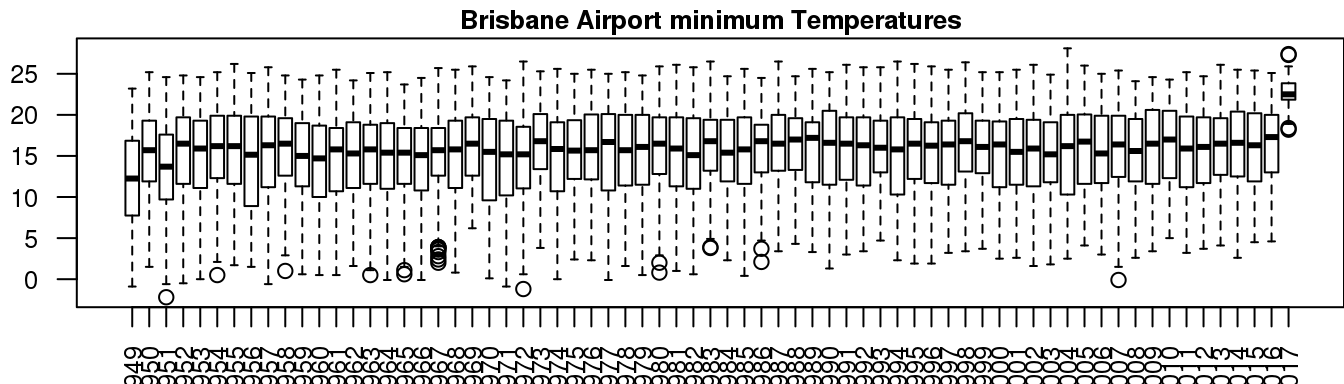
\includegraphics{intro-to-r_files/figure-latex/unnamed-chunk-77-1.pdf}

\begin{Shaded}
\begin{Highlighting}[]
\CommentTok{# This generates a boxplot of 1000 gene expression values for the first}
\CommentTok{# 15 samples. Remember, gene.atlas contains over 22,000 expression values}
\CommentTok{# and 158 samples}
\end{Highlighting}
\end{Shaded}

\subsection{ggplot2::geom\_boxplot()}\label{ggplot2geom_boxplot}

Using ggplot2 we can produce a much more attractive plot, although doing
so is considerably more complicated.

\begin{Shaded}
\begin{Highlighting}[]
\CommentTok{# Using ggplot, we first need to load the required libraries}
\KeywordTok{library}\NormalTok{(ggplot2)}
\KeywordTok{library}\NormalTok{(reshape2)}

\CommentTok{# Once again, get 1000 values for 15 samples}
\NormalTok{atlas.subset <-}\StringTok{ }\KeywordTok{as.data.frame}\NormalTok{(}\KeywordTok{t}\NormalTok{(}\KeywordTok{log2}\NormalTok{(gene.atlas[}\KeywordTok{sample}\NormalTok{(}\KeywordTok{nrow}\NormalTok{(gene.atlas), }\DecValTok{1000}\NormalTok{),}
                                                \KeywordTok{seq}\NormalTok{(}\DecValTok{15}\NormalTok{)])))}

\CommentTok{# We now need to transform the data from 'wide' to 'long' format}
\CommentTok{# Your instructor will explain this process}
\NormalTok{atlas.subset <-}\StringTok{ }\KeywordTok{cbind}\NormalTok{(atlas.subset,}\DataTypeTok{Group=}\KeywordTok{as.factor}\NormalTok{(}\KeywordTok{paste0}\NormalTok{(}\StringTok{"Group"}\NormalTok{,}\KeywordTok{rep}\NormalTok{(}\KeywordTok{seq}\NormalTok{(}\DecValTok{3}\NormalTok{), }\DecValTok{5}\NormalTok{))),}
                      \DataTypeTok{Sample=}\KeywordTok{rownames}\NormalTok{(atlas.subset))}
\NormalTok{atlas.melt <-}\StringTok{ }\KeywordTok{melt}\NormalTok{(atlas.subset,}
                   \DataTypeTok{id.vars=}\KeywordTok{c}\NormalTok{(}\StringTok{"Group"}\NormalTok{, }\StringTok{"Sample"}\NormalTok{),}
                   \DataTypeTok{variable.name=}\StringTok{"Gene"}\NormalTok{,}
                   \DataTypeTok{value.name=}\StringTok{"Signal"}\NormalTok{)}

\CommentTok{# Now that the data is in the correct format, we can draw the graph}
\CommentTok{# Again, the instructor will explain what is happening here}
\CommentTok{# The '+' symbols are required, and tell R that the command is not finished}
\NormalTok{p <-}\StringTok{ }\KeywordTok{ggplot}\NormalTok{(atlas.melt, }\KeywordTok{aes}\NormalTok{(}\KeywordTok{factor}\NormalTok{(Sample), Signal, }\DataTypeTok{fill=}\NormalTok{Group)) +}\StringTok{ }
\StringTok{  }\KeywordTok{geom_boxplot}\NormalTok{() +}\StringTok{ }
\StringTok{  }\KeywordTok{labs}\NormalTok{(}\DataTypeTok{title=}\StringTok{"boxplot summarising signal intensity"}\NormalTok{, }\DataTypeTok{x=}\StringTok{"array"}\NormalTok{, }\DataTypeTok{y=}\StringTok{"log2 signal"}\NormalTok{) +}\StringTok{ }
\StringTok{  }\KeywordTok{theme}\NormalTok{(}\DataTypeTok{axis.text.x=}\KeywordTok{element_text}\NormalTok{(}\DataTypeTok{angle=}\DecValTok{90}\NormalTok{))}
\KeywordTok{print}\NormalTok{(p)}
\end{Highlighting}
\end{Shaded}

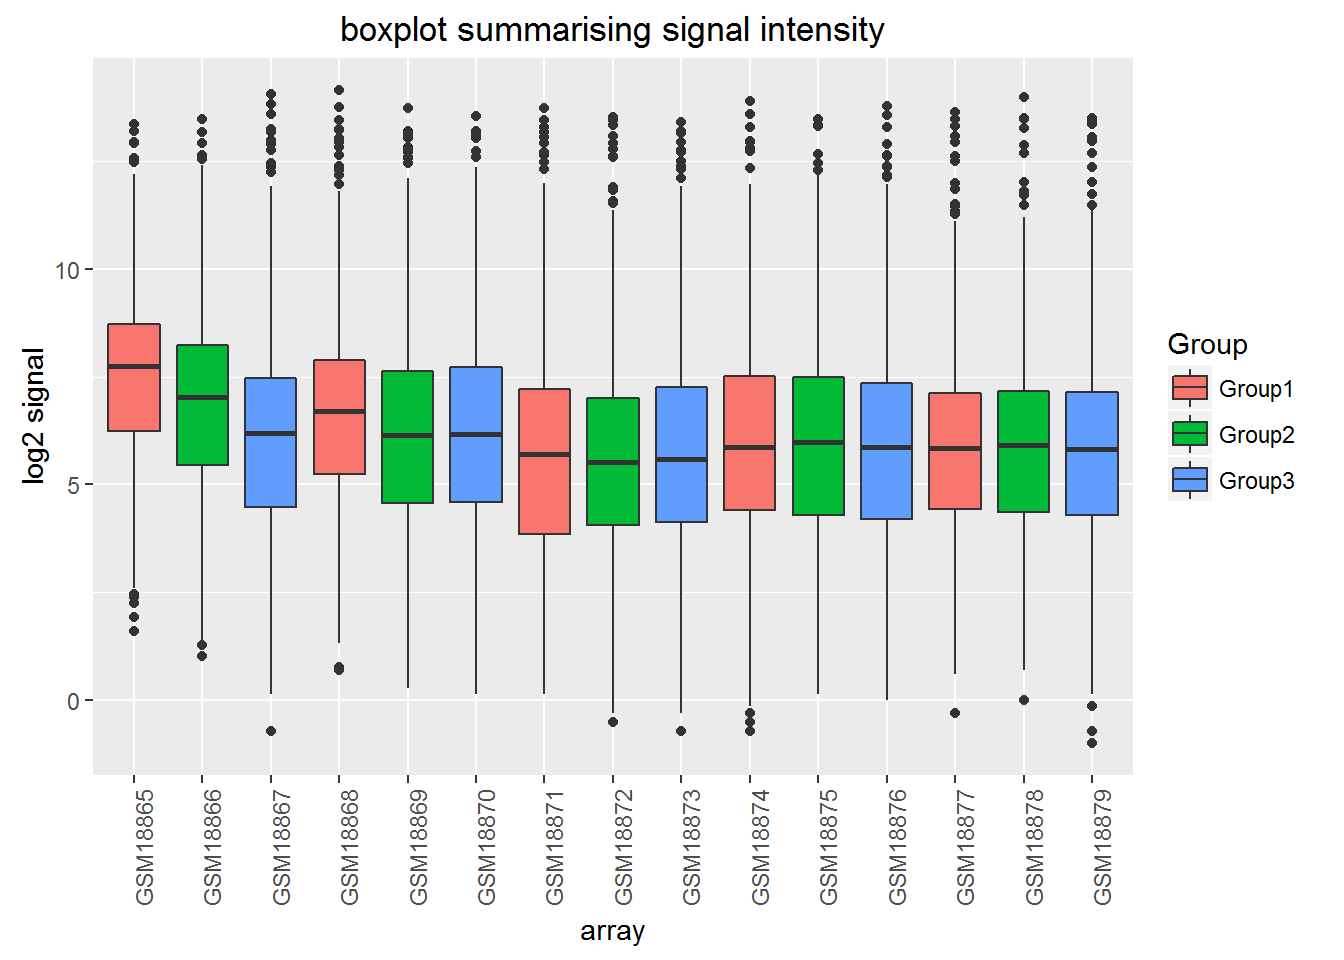
\includegraphics{intro-to-r_files/figure-latex/unnamed-chunk-78-1.pdf}

\section{Histograms}\label{histograms}

A histogram shows the distribution of data for typically a single
sample.

\subsection{Native}\label{native-1}

Let's use the same data that we used in the boxplot example but
concentrating on the signal intensity for the first sample only.

\begin{Shaded}
\begin{Highlighting}[]
\CommentTok{# The base graphics way}
\CommentTok{# Create a data frame slice containing our target expression data}
\NormalTok{channel.data <-}\StringTok{ }\KeywordTok{data.frame}\NormalTok{(}\DataTypeTok{Signal=}\KeywordTok{log2}\NormalTok{(gene.atlas[}\KeywordTok{sample}\NormalTok{(}\KeywordTok{nrow}\NormalTok{(gene.atlas),}\DecValTok{1000}\NormalTok{),}\DecValTok{1}\NormalTok{]))}

\CommentTok{# hist() is the built-in histogram function}
\CommentTok{# [, 1] selects the first (and in this case, only) column of data from channel.data}
\KeywordTok{hist}\NormalTok{(channel.data[, }\DecValTok{1}\NormalTok{])}
\end{Highlighting}
\end{Shaded}

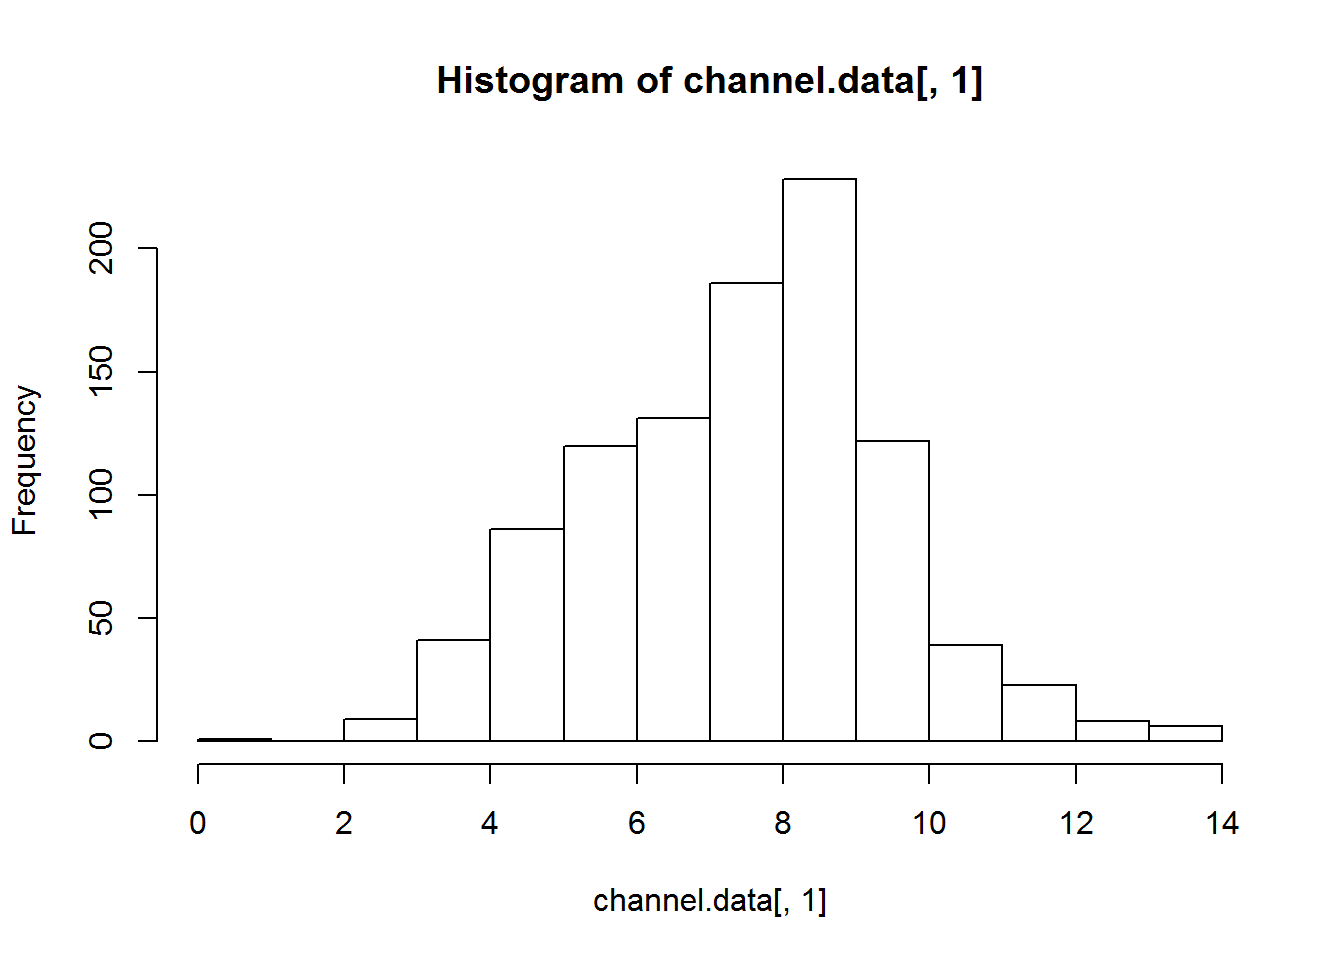
\includegraphics{intro-to-r_files/figure-latex/unnamed-chunk-79-1.pdf}

\subsection{ggplot2 - geom\_histogram()}\label{ggplot2---geom_histogram}

\begin{Shaded}
\begin{Highlighting}[]
\CommentTok{# Now with ggplot2. The data is already in long format, so no need to 'melt'}
\CommentTok{# this time. Also ggplot2 is already loaded, so no need to do that again.}
\NormalTok{p <-}\StringTok{ }\KeywordTok{ggplot}\NormalTok{(channel.data, }\KeywordTok{aes}\NormalTok{(}\DataTypeTok{x=}\NormalTok{Signal)) +}\StringTok{ }
\StringTok{  }\KeywordTok{geom_histogram}\NormalTok{(}\DataTypeTok{binwidth=}\FloatTok{0.2}\NormalTok{) +}
\StringTok{  }\KeywordTok{labs}\NormalTok{(}\DataTypeTok{title=}\StringTok{"Histogram summarising signal intensity for sample 1"}\NormalTok{)}
\KeywordTok{print}\NormalTok{(p)}
\end{Highlighting}
\end{Shaded}

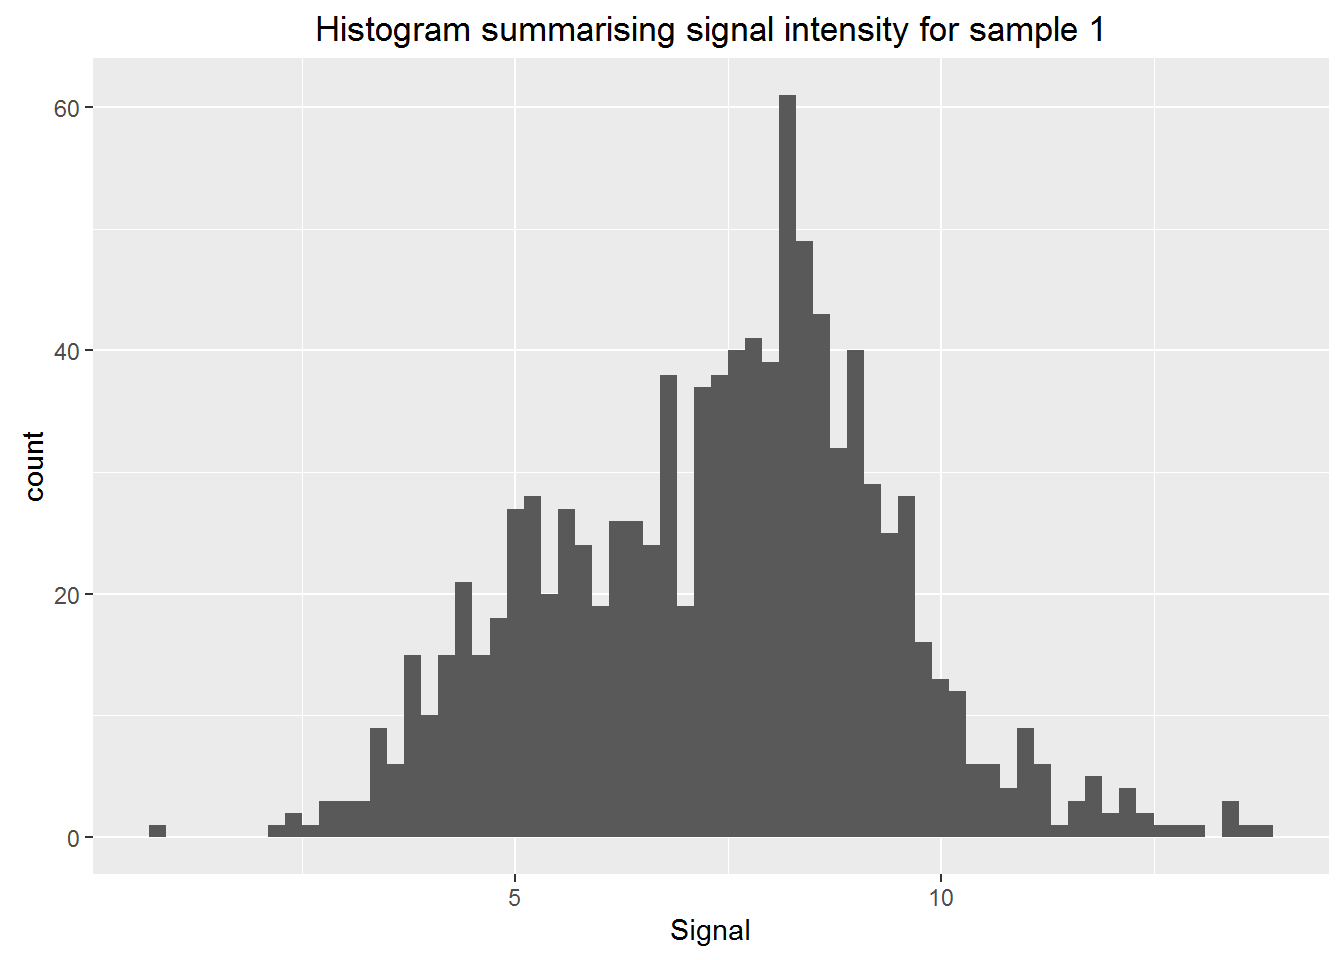
\includegraphics{intro-to-r_files/figure-latex/unnamed-chunk-80-1.pdf}

\begin{rmdtip}
See also \texttt{plot(density())} for a more continuous view of the data
distribution.
\end{rmdtip}

\section{Bar charts}\label{bar-charts}

A barchart is superficially similar to a histogram in the bars of data
are displayed. Bar charts are ideal for displaying counts associated
with categorical data.

\subsection{Native}\label{native-2}

The example chart here simply presents the number of diamonds in a
database of diamonds that have bheen assigned to particular classes of
cut. The diamonds data comes from one of the many datasets built into R
that you can use for testing and experimentation. For a full list of
these, use \texttt{library(help="datasets")}.

\begin{Shaded}
\begin{Highlighting}[]
\CommentTok{# Let's start by having a look at the data}
\KeywordTok{head}\NormalTok{(diamonds)}
\end{Highlighting}
\end{Shaded}

\begin{verbatim}
## # A tibble: 6 x 10
##   carat       cut color clarity depth table price     x     y     z
##   <dbl>     <ord> <ord>   <ord> <dbl> <dbl> <int> <dbl> <dbl> <dbl>
## 1  0.23     Ideal     E     SI2  61.5    55   326  3.95  3.98  2.43
## 2  0.21   Premium     E     SI1  59.8    61   326  3.89  3.84  2.31
## 3  0.23      Good     E     VS1  56.9    65   327  4.05  4.07  2.31
## 4  0.29   Premium     I     VS2  62.4    58   334  4.20  4.23  2.63
## 5  0.31      Good     J     SI2  63.3    58   335  4.34  4.35  2.75
## 6  0.24 Very Good     J    VVS2  62.8    57   336  3.94  3.96  2.48
\end{verbatim}

\begin{Shaded}
\begin{Highlighting}[]
\KeywordTok{str}\NormalTok{(diamonds)}
\end{Highlighting}
\end{Shaded}

\begin{verbatim}
## Classes 'tbl_df', 'tbl' and 'data.frame':    53940 obs. of  10 variables:
##  $ carat  : num  0.23 0.21 0.23 0.29 0.31 0.24 0.24 0.26 0.22 0.23 ...
##  $ cut    : Ord.factor w/ 5 levels "Fair"<"Good"<..: 5 4 2 4 2 3 3 3 1 3 ...
##  $ color  : Ord.factor w/ 7 levels "D"<"E"<"F"<"G"<..: 2 2 2 6 7 7 6 5 2 5 ...
##  $ clarity: Ord.factor w/ 8 levels "I1"<"SI2"<"SI1"<..: 2 3 5 4 2 6 7 3 4 5 ...
##  $ depth  : num  61.5 59.8 56.9 62.4 63.3 62.8 62.3 61.9 65.1 59.4 ...
##  $ table  : num  55 61 65 58 58 57 57 55 61 61 ...
##  $ price  : int  326 326 327 334 335 336 336 337 337 338 ...
##  $ x      : num  3.95 3.89 4.05 4.2 4.34 3.94 3.95 4.07 3.87 4 ...
##  $ y      : num  3.98 3.84 4.07 4.23 4.35 3.96 3.98 4.11 3.78 4.05 ...
##  $ z      : num  2.43 2.31 2.31 2.63 2.75 2.48 2.47 2.53 2.49 2.39 ...
\end{verbatim}

\begin{Shaded}
\begin{Highlighting}[]
\CommentTok{# Barplot using base version of barplot, grouping by the 'cut' category}
\KeywordTok{barplot}\NormalTok{(}\KeywordTok{table}\NormalTok{(diamonds[,}\StringTok{"cut"}\NormalTok{]))}
\end{Highlighting}
\end{Shaded}

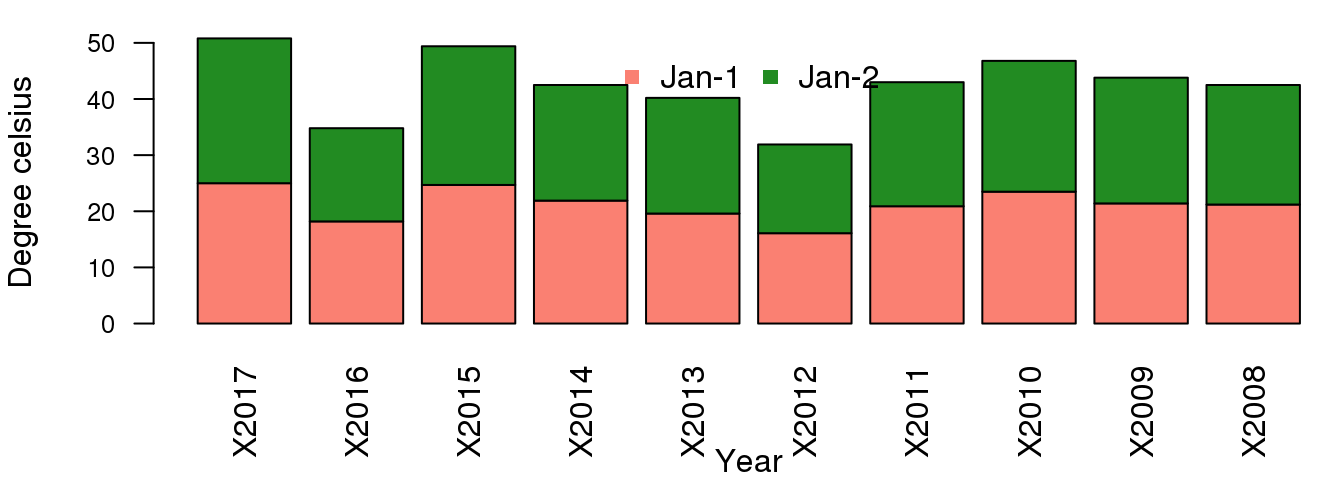
\includegraphics{intro-to-r_files/figure-latex/unnamed-chunk-82-1.pdf}

\subsection{ggplot2::geom\_bar()}\label{ggplot2geom_bar}

\begin{Shaded}
\begin{Highlighting}[]
\CommentTok{# The ggplot version in this case can be quite simple. This is thanks to the}
\CommentTok{# data again being in long format, so not needing melting}
\NormalTok{p <-}\StringTok{ }\KeywordTok{ggplot}\NormalTok{(diamonds, }\KeywordTok{aes}\NormalTok{(cut)) +}\StringTok{ }\KeywordTok{geom_bar}\NormalTok{()}
\KeywordTok{print}\NormalTok{(p)}
\end{Highlighting}
\end{Shaded}

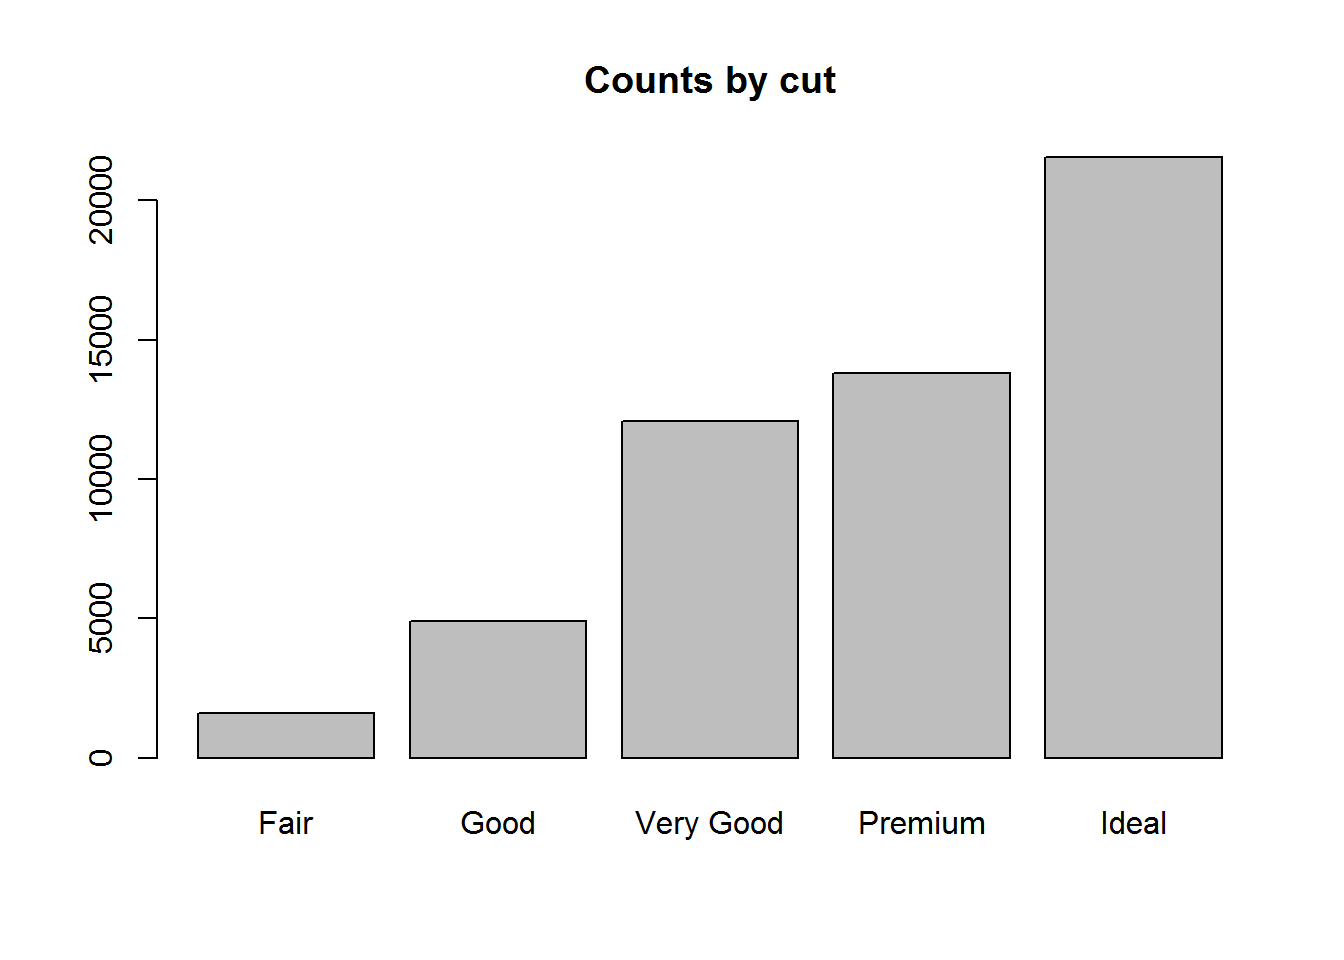
\includegraphics{intro-to-r_files/figure-latex/unnamed-chunk-83-1.pdf}

\begin{Shaded}
\begin{Highlighting}[]
\CommentTok{# Similarly, group by 'color' (and appropriately enough, let's colour it in}
\CommentTok{# this time)}
\NormalTok{p <-}\StringTok{ }\KeywordTok{ggplot}\NormalTok{(diamonds, }\KeywordTok{aes}\NormalTok{(color, }\DataTypeTok{fill =} \NormalTok{color)) +}\StringTok{ }\KeywordTok{geom_bar}\NormalTok{()}
\KeywordTok{print}\NormalTok{(p)}
\end{Highlighting}
\end{Shaded}

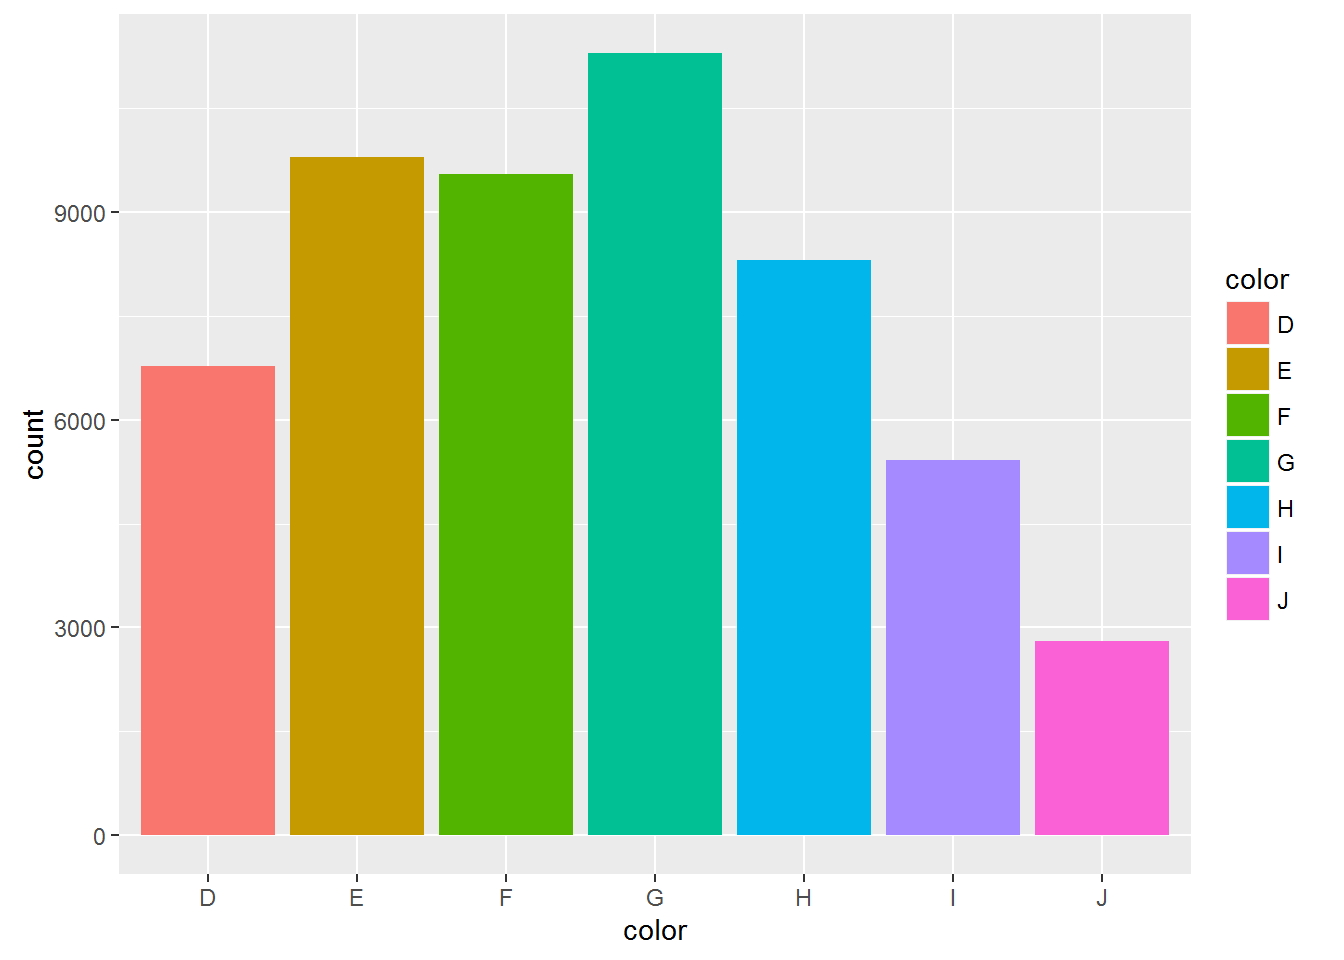
\includegraphics{intro-to-r_files/figure-latex/unnamed-chunk-83-2.pdf}

\section{Scatterplots}\label{scatterplots}

Scatterplots are widely used for plotting data where an object has
mutiple variables.

\subsection{Native}\label{native-3}

The iris dataset, another built-in dataset in R, describes three
varieties of the iris flower and a number of attributes that include the
sepal and petal lengths and widths. In this case we are going to plot
sepal length against width for three species of iris.

\begin{Shaded}
\begin{Highlighting}[]
\KeywordTok{head}\NormalTok{(iris)}
\end{Highlighting}
\end{Shaded}

\begin{verbatim}
##   Sepal.Length Sepal.Width Petal.Length Petal.Width Species
## 1          5.1         3.5          1.4         0.2  setosa
## 2          4.9         3.0          1.4         0.2  setosa
## 3          4.7         3.2          1.3         0.2  setosa
## 4          4.6         3.1          1.5         0.2  setosa
## 5          5.0         3.6          1.4         0.2  setosa
## 6          5.4         3.9          1.7         0.4  setosa
\end{verbatim}

\begin{Shaded}
\begin{Highlighting}[]
\KeywordTok{str}\NormalTok{(iris)}
\end{Highlighting}
\end{Shaded}

\begin{verbatim}
## 'data.frame':    150 obs. of  5 variables:
##  $ Sepal.Length: num  5.1 4.9 4.7 4.6 5 5.4 4.6 5 4.4 4.9 ...
##  $ Sepal.Width : num  3.5 3 3.2 3.1 3.6 3.9 3.4 3.4 2.9 3.1 ...
##  $ Petal.Length: num  1.4 1.4 1.3 1.5 1.4 1.7 1.4 1.5 1.4 1.5 ...
##  $ Petal.Width : num  0.2 0.2 0.2 0.2 0.2 0.4 0.3 0.2 0.2 0.1 ...
##  $ Species     : Factor w/ 3 levels "setosa","versicolor",..: 1 1 1 1 1 1 1 1 1 1 ...
\end{verbatim}

\begin{Shaded}
\begin{Highlighting}[]
\CommentTok{# Base graphics. But there is no easy way with this to distinguish the}
\CommentTok{# three species, so the data is pretty much useless}
\KeywordTok{plot}\NormalTok{(iris[,}\StringTok{"Sepal.Length"}\NormalTok{], iris[,}\StringTok{"Sepal.Width"}\NormalTok{])}
\end{Highlighting}
\end{Shaded}

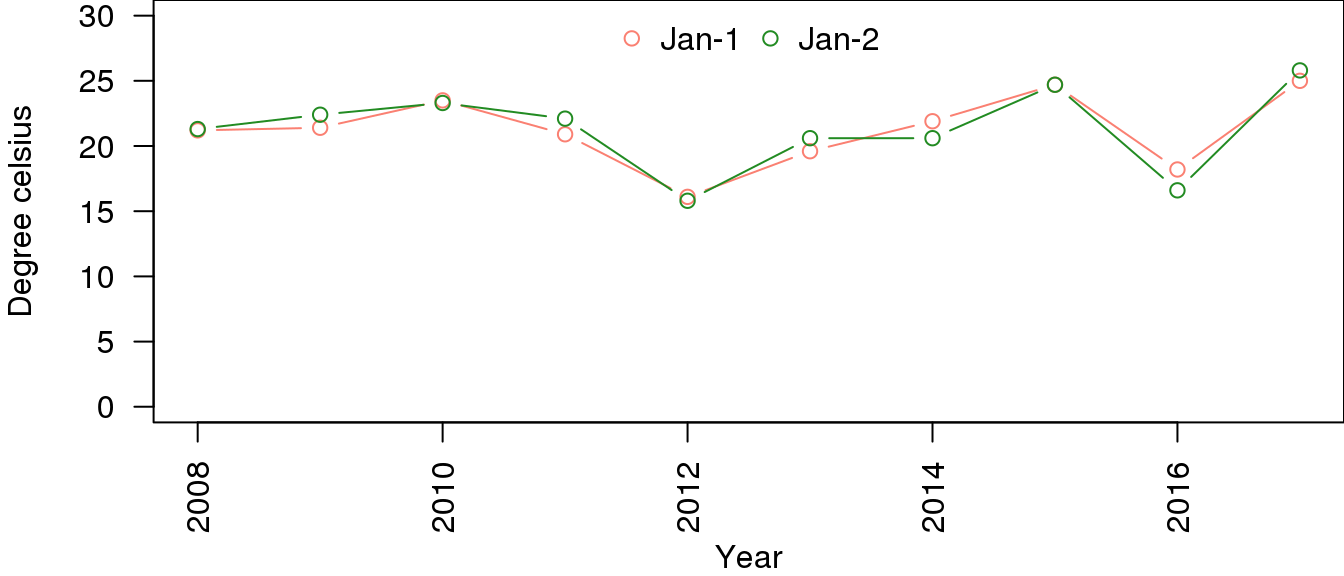
\includegraphics{intro-to-r_files/figure-latex/unnamed-chunk-84-1.pdf}

\subsection{ggplot2::geom\_point()}\label{ggplot2geom_point}

\begin{Shaded}
\begin{Highlighting}[]
\CommentTok{# With ggplot, we can specify that we want to colour the points by Species}
\NormalTok{p <-}\StringTok{ }\KeywordTok{ggplot}\NormalTok{(iris, }\KeywordTok{aes}\NormalTok{(Sepal.Length, Sepal.Width)) +}\StringTok{ }
\StringTok{  }\KeywordTok{geom_point}\NormalTok{(}\KeywordTok{aes}\NormalTok{(}\DataTypeTok{color =} \NormalTok{Species), }\DataTypeTok{size=}\DecValTok{3}\NormalTok{)}
\KeywordTok{print}\NormalTok{(p)}
\end{Highlighting}
\end{Shaded}

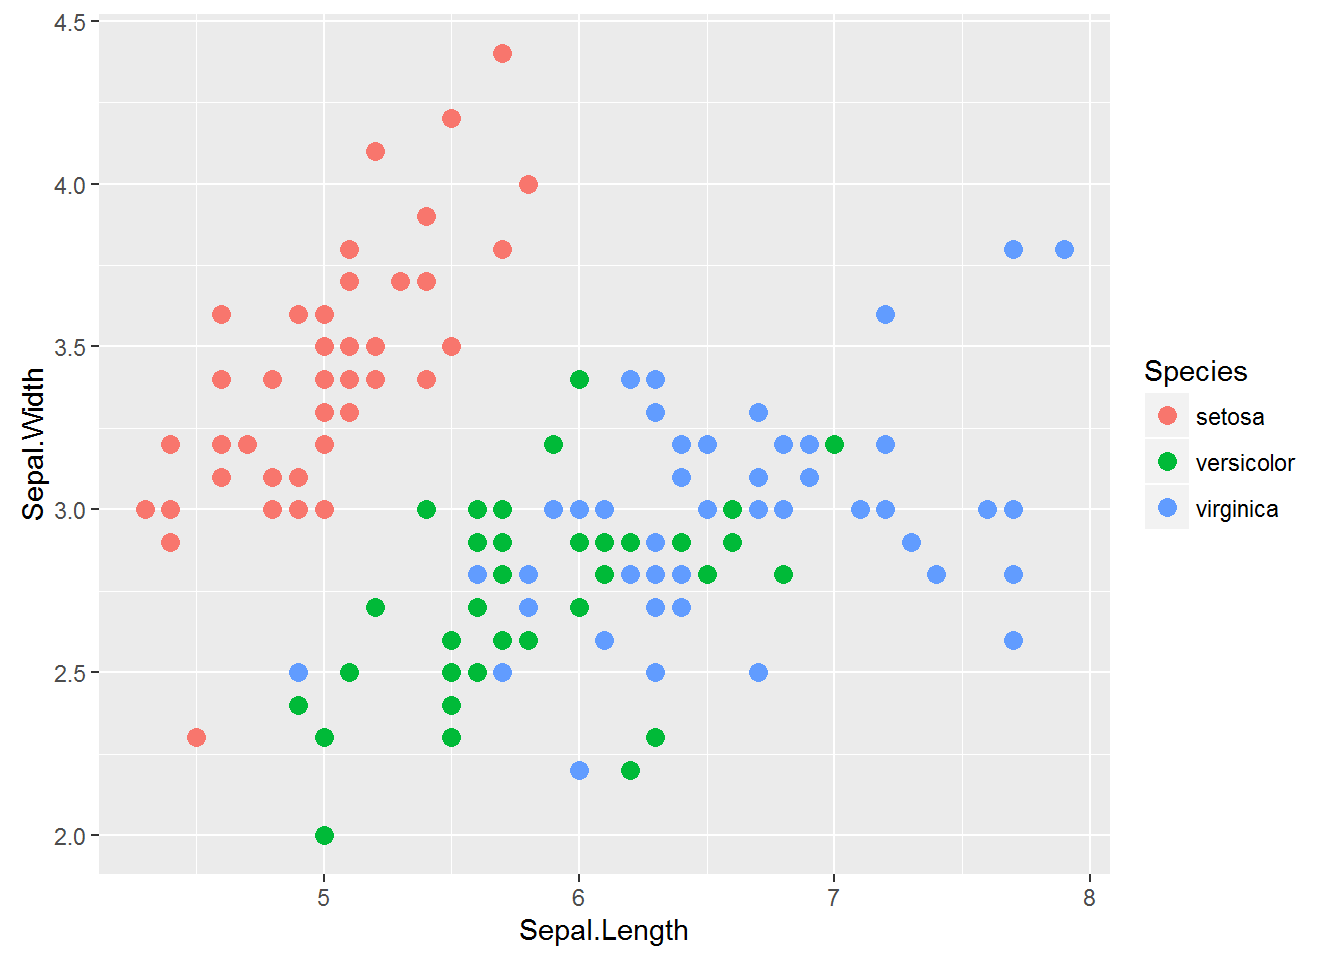
\includegraphics{intro-to-r_files/figure-latex/unnamed-chunk-85-1.pdf}

Now the variation in sepal shape between the species is clear

\begin{rmdexercise}
\textbf{Plotting with R}

Work your way through the previous code examples to draw boxplots,
histograms, bar charts and scatter plots as described. In each case, the
built-in plot function is described first, then the \texttt{ggplot2}
version.
\end{rmdexercise}

\section{Venn Diagrams}\label{venn-diagrams}

The Venn diagram is a useful plot for describing sets of information and
can reflect the intersections of data. There are a number of packages
that can be used for preparing Venn diagrams. I would recommend the
''Vennerable'' package which can be downloaded from R-forge. This is not
quite as comprehensive or complete in functionality compared to other
packages but it the easiest to use and implement by a wide margin.

\begin{Shaded}
\begin{Highlighting}[]
\CommentTok{# Vennerable is already installed on the training server, but you might need to}
\CommentTok{# install it before use with another R instance}
\CommentTok{# install.packages("Vennerable", repos="http://R-Forge.R-project.org")}
\CommentTok{# Although it's installed, it's not loaded until we tell R to do so}
\KeywordTok{library}\NormalTok{(Vennerable)}

\CommentTok{# Like the R base install, Vennerable comes with built-in test data, in the}
\CommentTok{# form of Stem Cell information. This is not automatically available though,}
\CommentTok{# so we need to load it}
\KeywordTok{data}\NormalTok{(StemCell)}

\CommentTok{# What does StemCell contain}
\KeywordTok{str}\NormalTok{(StemCell)}
\end{Highlighting}
\end{Shaded}

\begin{Shaded}
\begin{Highlighting}[]
\CommentTok{# It is a list of four character vectors, giving a list of the genes expressed}
\CommentTok{# in each of four types of stem cell}
\CommentTok{# Use the Venn function to count overlap between the lists}
\NormalTok{Vstem <-}\StringTok{ }\KeywordTok{Venn}\NormalTok{(StemCell)}
\NormalTok{Vstem}
\end{Highlighting}
\end{Shaded}

\begin{Shaded}
\begin{Highlighting}[]
\CommentTok{# And plot a venn diagram of those overlaps}
\KeywordTok{plot}\NormalTok{(Vstem, }\DataTypeTok{type=}\StringTok{"ellipses"}\NormalTok{, }\DataTypeTok{doWeights=}\OtherTok{FALSE}\NormalTok{)}
\end{Highlighting}
\end{Shaded}

\begin{rmdexercise}
\textbf{Venn Diagrams}

\begin{enumerate}
\def\labelenumi{\arabic{enumi}.}
\tightlist
\item
  Draw a Venn diagram using the code above
\item
  Explore the Vennerable vignette (use Google to find it online) and try
  designing some differently-formatted venn diagrams
\item
  How many genes are expressed in all four cell types? Can you retrieve
  their Gene IDs from the Vstem object?
\end{enumerate}
\end{rmdexercise}

\chapter*{Appendix 1}\label{appendix-1}
\addcontentsline{toc}{chapter}{Appendix 1}

\section*{Summary of Object Types}\label{summary-of-object-types}
\addcontentsline{toc}{section}{Summary of Object Types}

\begin{longtable}[]{@{}ll@{}}
\toprule
\begin{minipage}[b]{0.09\columnwidth}\raggedright\strut
Type\strut
\end{minipage} & \begin{minipage}[b]{0.72\columnwidth}\raggedright\strut
Description\strut
\end{minipage}\tabularnewline
\midrule
\endhead
\begin{minipage}[t]{0.09\columnwidth}\raggedright\strut
\textbf{vectors}\strut
\end{minipage} & \begin{minipage}[t]{0.72\columnwidth}\raggedright\strut
ordered collection of numeric, character, complex and logical
values.\strut
\end{minipage}\tabularnewline
\begin{minipage}[t]{0.09\columnwidth}\raggedright\strut
\textbf{factors}\strut
\end{minipage} & \begin{minipage}[t]{0.72\columnwidth}\raggedright\strut
special type vectors with grouping information of its components\strut
\end{minipage}\tabularnewline
\begin{minipage}[t]{0.09\columnwidth}\raggedright\strut
\textbf{data frames}\strut
\end{minipage} & \begin{minipage}[t]{0.72\columnwidth}\raggedright\strut
two dimensional structures with different data types\strut
\end{minipage}\tabularnewline
\begin{minipage}[t]{0.09\columnwidth}\raggedright\strut
\textbf{matrices}\strut
\end{minipage} & \begin{minipage}[t]{0.72\columnwidth}\raggedright\strut
two dimensional structures with data of same type\strut
\end{minipage}\tabularnewline
\begin{minipage}[t]{0.09\columnwidth}\raggedright\strut
\textbf{arrays}\strut
\end{minipage} & \begin{minipage}[t]{0.72\columnwidth}\raggedright\strut
multidimensional arrays of vectors\strut
\end{minipage}\tabularnewline
\begin{minipage}[t]{0.09\columnwidth}\raggedright\strut
\textbf{lists}\strut
\end{minipage} & \begin{minipage}[t]{0.72\columnwidth}\raggedright\strut
general form of vectors with different types of elements\strut
\end{minipage}\tabularnewline
\begin{minipage}[t]{0.09\columnwidth}\raggedright\strut
\textbf{functions}\strut
\end{minipage} & \begin{minipage}[t]{0.72\columnwidth}\raggedright\strut
piece of code\strut
\end{minipage}\tabularnewline
\bottomrule
\end{longtable}

\section*{More information on R and Bioconductor for
Genomics}\label{more-information-on-r-and-bioconductor-for-genomics}
\addcontentsline{toc}{section}{More information on R and Bioconductor
for Genomics}

\begin{itemize}
\tightlist
\item
  Thomas Girke's manuals and guides to R
  \url{http://manuals.bioinformatics.ucr.edu/home}
\item
  \url{http://www.r-bloggers.com/}
\end{itemize}

\chapter*{Appendix 2 - Solutions to
exercises}\label{appendix-2---solutions-to-exercises}
\addcontentsline{toc}{chapter}{Appendix 2 - Solutions to exercises}

\section*{2.4.1 Using vectors}\label{using-vectors}
\addcontentsline{toc}{section}{2.4.1 Using vectors}

\texttt{mixedVector{[}2{]}} returns the name and value of the second
element of the vector.

\texttt{mixedVector{[}{[}2{]}{]}} just returns the value

\begin{Shaded}
\begin{Highlighting}[]
\NormalTok{mixedVector[[}\StringTok{'meaningOfLife'}\NormalTok{]]}
\end{Highlighting}
\end{Shaded}

\section*{2.4.3 Using lists}\label{using-lists}
\addcontentsline{toc}{section}{2.4.3 Using lists}

\begin{Shaded}
\begin{Highlighting}[]
\CommentTok{# Retrieve second and fourth elements}
\NormalTok{mixedList[}\KeywordTok{c}\NormalTok{(}\DecValTok{2}\NormalTok{,}\DecValTok{4}\NormalTok{)]}

\CommentTok{# Retrive everything BUT 2nd and 4th elements}
\NormalTok{mixedList[}\KeywordTok{c}\NormalTok{(-}\DecValTok{2}\NormalTok{,-}\DecValTok{4}\NormalTok{)]}
\NormalTok{names <-}\StringTok{ }\KeywordTok{c}\NormalTok{(}\StringTok{"A"}\NormalTok{, }\StringTok{"B"}\NormalTok{, }\StringTok{"C"}\NormalTok{, }\StringTok{"D"}\NormalTok{, }\StringTok{"E"}\NormalTok{, }\StringTok{"F"}\NormalTok{, }\StringTok{"G"}\NormalTok{, }\StringTok{"H"}\NormalTok{, }\StringTok{"I"}\NormalTok{, }\StringTok{"J"}\NormalTok{)}
\NormalTok{sex <-}\StringTok{ }\KeywordTok{c}\NormalTok{(}\OtherTok{TRUE}\NormalTok{, }\OtherTok{TRUE}\NormalTok{, }\OtherTok{TRUE}\NormalTok{, }\OtherTok{TRUE}\NormalTok{, }\OtherTok{TRUE}\NormalTok{, }\OtherTok{FALSE}\NormalTok{, }\OtherTok{FALSE}\NormalTok{, }\OtherTok{FALSE}\NormalTok{, }\OtherTok{FALSE}\NormalTok{, }\OtherTok{FALSE}\NormalTok{)}
\NormalTok{age <-}\StringTok{ }\KeywordTok{c}\NormalTok{(}\DecValTok{1}\NormalTok{,}\DecValTok{2}\NormalTok{,}\DecValTok{3}\NormalTok{,}\DecValTok{4}\NormalTok{,}\DecValTok{5}\NormalTok{,}\DecValTok{6}\NormalTok{,}\DecValTok{7}\NormalTok{,}\DecValTok{8}\NormalTok{,}\DecValTok{9}\NormalTok{,}\DecValTok{10}\NormalTok{)}
\NormalTok{subjects <-}\StringTok{ }\KeywordTok{list}\NormalTok{(}\DataTypeTok{names=}\NormalTok{names, }\DataTypeTok{sex=}\NormalTok{sex, }\DataTypeTok{age=}\NormalTok{age)}
\end{Highlighting}
\end{Shaded}

\section*{2.4.4 Adding factor values}\label{adding-factor-values}
\addcontentsline{toc}{section}{2.4.4 Adding factor values}

\begin{Shaded}
\begin{Highlighting}[]
\KeywordTok{levels}\NormalTok{(mandm) <-}\StringTok{ }\KeywordTok{c}\NormalTok{(}\KeywordTok{levels}\NormalTok{(mandm), }\StringTok{"brown"}\NormalTok{)}

\CommentTok{# Change vector values 100 to 200 to brown}
\NormalTok{mandm[}\DecValTok{100}\NormalTok{:}\DecValTok{200}\NormalTok{] =}\StringTok{ 'brown'}
\end{Highlighting}
\end{Shaded}

\section*{2.4.6 Creating a data frame}\label{creating-a-data-frame}
\addcontentsline{toc}{section}{2.4.6 Creating a data frame}

\begin{Shaded}
\begin{Highlighting}[]
\NormalTok{subject.data <-}\StringTok{ }\KeywordTok{as.data.frame}\NormalTok{(subjects)}
\KeywordTok{colnames}\NormalTok{(subject.data)}

\CommentTok{# If they need naming}
\KeywordTok{colnames}\NormalTok{(subject.data) <-}\StringTok{ }\KeywordTok{c}\NormalTok{(}\StringTok{'names'}\NormalTok{,}\StringTok{'sex'}\NormalTok{,}\StringTok{'age'}\NormalTok{)}
\end{Highlighting}
\end{Shaded}

\section*{4.2 Reading in the GeneAtlas
data}\label{reading-in-the-geneatlas-data}
\addcontentsline{toc}{section}{4.2 Reading in the GeneAtlas data}

\begin{Shaded}
\begin{Highlighting}[]
\CommentTok{# note the the comment/metadata delimiter is the ! symbol}
\CommentTok{# the column values are separated by tabs}
\CommentTok{# the column names are included in the first row - we can import Header}
\KeywordTok{head}\NormalTok{(}\KeywordTok{read.table}\NormalTok{(gene.atlas.file, }\DataTypeTok{comment.char=}\StringTok{"!"} \DataTypeTok{sep=}\StringTok{"}\CharTok{\textbackslash{}t}\StringTok{"}\NormalTok{, }\DataTypeTok{header=}\OtherTok{TRUE}\NormalTok{))}
\NormalTok{gene.atlas <-}\StringTok{ }\KeywordTok{read.table}\NormalTok{(gene.atlas.file, }\DataTypeTok{comment.char=}\StringTok{"!"}\NormalTok{, }\DataTypeTok{sep=}\StringTok{"}\CharTok{\textbackslash{}t}\StringTok{"}\NormalTok{, }\DataTypeTok{header=}\OtherTok{TRUE}\NormalTok{)}

\CommentTok{# read the data again, this time set the row.names with the first data column}
\NormalTok{gene.atlas <-}\StringTok{ }\KeywordTok{read.table}\NormalTok{(gene.atlas.file, }\DataTypeTok{comment.char=}\StringTok{"!"}\NormalTok{, }\DataTypeTok{sep=}\StringTok{"}\CharTok{\textbackslash{}t}\StringTok{"}\NormalTok{,}
                         \DataTypeTok{header=}\OtherTok{TRUE}\NormalTok{, }\DataTypeTok{row.names=}\DecValTok{1}\NormalTok{)}
\end{Highlighting}
\end{Shaded}

\section*{5.1 Creating and using
functions}\label{creating-and-using-functions}
\addcontentsline{toc}{section}{5.1 Creating and using functions}

\begin{Shaded}
\begin{Highlighting}[]
\CommentTok{# A function to multiply or divide}
\NormalTok{multiplyFunction <-}\StringTok{ }\NormalTok{function(a, }\DataTypeTok{b=}\DecValTok{2}\NormalTok{, }\DataTypeTok{multiply=}\OtherTok{TRUE}\NormalTok{) \{}
  \NormalTok{if (multiply) \{}
    \NormalTok{a*b}
  \NormalTok{\} else \{}
    \NormalTok{a/b}
  \NormalTok{\}}
\NormalTok{\}}

\CommentTok{# A function to return a letter at a certain position}
\NormalTok{letterFunction <-}\StringTok{ }\NormalTok{function(word, position) \{}
  \KeywordTok{substr}\NormalTok{(word, position, position)}
\NormalTok{\}}

\CommentTok{# A function to generate a filled matrix}
\NormalTok{makeMatrix <-}\StringTok{ }\NormalTok{function (rows, columns, }\DataTypeTok{numbers =} \OtherTok{TRUE}\NormalTok{) \{}
  \NormalTok{if (numbers) \{}
    \KeywordTok{matrix}\NormalTok{(}\KeywordTok{seq}\NormalTok{(rows*columns), }\DataTypeTok{nrow =} \NormalTok{rows, }\DataTypeTok{ncol =} \NormalTok{columns)}
  \NormalTok{\} else \{}
    \KeywordTok{matrix}\NormalTok{(LETTERS[}\DecValTok{1}\NormalTok{:(rows*columns)], }\DataTypeTok{nrow =} \NormalTok{rows, }\DataTypeTok{ncol =} \NormalTok{columns)}
  \NormalTok{\}}
\NormalTok{\}}
\end{Highlighting}
\end{Shaded}

\section*{5.2 Loops and vectorisation}\label{loops-and-vectorisation}
\addcontentsline{toc}{section}{5.2 Loops and vectorisation}

\begin{Shaded}
\begin{Highlighting}[]
\CommentTok{# Count down from 100 in 2s}
\NormalTok{i <-}\StringTok{ }\DecValTok{100}
\NormalTok{while (i >=}\StringTok{ }\DecValTok{0}\NormalTok{) \{}
  \KeywordTok{print}\NormalTok{(i)}
  \NormalTok{i<<-i}\DecValTok{-2}
\NormalTok{\}}

\CommentTok{# Square of the numbers from 1 to 20}
\NormalTok{startVec <-}\StringTok{ }\KeywordTok{seq}\NormalTok{(}\DecValTok{20}\NormalTok{)}
\NormalTok{squareVec <-}\StringTok{ }\NormalTok{startVec^}\DecValTok{2}
\end{Highlighting}
\end{Shaded}

\section*{6.5 Venn diagram}\label{venn-diagram}
\addcontentsline{toc}{section}{6.5 Venn diagram}

\begin{Shaded}
\begin{Highlighting}[]
\KeywordTok{str}\NormalTok{(Vstem)}
\NormalTok{Vstem@IntersectionSets$}\StringTok{"1111"}
\end{Highlighting}
\end{Shaded}

\chapter*{Appendix 3 - The SessionInfo for this version
of}\label{appendix-3---the-sessioninfo-for-this-version-of}
\addcontentsline{toc}{chapter}{Appendix 3 - The SessionInfo for this
version of}

\begin{Shaded}
\begin{Highlighting}[]
\KeywordTok{sessionInfo}\NormalTok{()}
\end{Highlighting}
\end{Shaded}

\begin{verbatim}
## R version 3.3.0 (2016-05-03)
## Platform: x86_64-w64-mingw32/x64 (64-bit)
## Running under: Windows 10 x64 (build 10240)
## 
## locale:
## [1] LC_COLLATE=English_Australia.1252  LC_CTYPE=English_Australia.1252   
## [3] LC_MONETARY=English_Australia.1252 LC_NUMERIC=C                      
## [5] LC_TIME=English_Australia.1252    
## 
## attached base packages:
## [1] stats     graphics  grDevices utils     datasets  methods   base     
## 
## other attached packages:
## [1] reshape2_1.4.1 ggplot2_2.1.0 
## 
## loaded via a namespace (and not attached):
##  [1] Rcpp_0.12.5        rstudioapi_0.6     knitr_1.14        
##  [4] magrittr_1.5       munsell_0.4.3      colorspace_1.2-6  
##  [7] xtable_1.8-2       R6_2.1.3           plyr_1.8.3        
## [10] stringr_1.0.0      tools_3.3.0        grid_3.3.0        
## [13] gtable_0.2.0       miniUI_0.1.1       htmltools_0.3.5   
## [16] yaml_2.1.13        assertthat_0.1     digest_0.6.9      
## [19] tibble_1.1         bookdown_0.1.5     shiny_0.13.2      
## [22] formatR_1.4        evaluate_0.9       mime_0.4          
## [25] rmarkdown_1.0.9008 labeling_0.3       stringi_1.1.1     
## [28] scales_0.4.0       httpuv_1.3.3
\end{verbatim}


\end{document}
